%!TEX program = xelatex
\documentclass[UTF8,fontset=fandol,11pt,a4paper]{ctexart}
\usepackage[margin=2.4cm]{geometry}
\usepackage{amsmath,amssymb,booktabs,graphicx,float,tabularx,array,multirow,makecell,threeparttable}
\usepackage{caption,subfigure,setspace,fancyhdr,chngcntr}
\usepackage[numbers,sort&compress]{natbib}
\usepackage[hidelinks,unicode]{hyperref}
\hypersetup{pdftitle={股指波动率预测与动态误差修正},pdfauthor={Boursin Nickel},pdfsubject={Public research revision; original content CC BY 4.0}}
\setstretch{1.35}\setlength{\headheight}{15pt}
\pagestyle{fancy}\fancyhf{}\fancyhead[C]{股指波动率预测与动态误差修正}\fancyfoot[C]{\thepage}
\counterwithin{table}{section}\counterwithin{figure}{section}\counterwithin{equation}{section}
\setlength{\emergencystretch}{3em}
\begin{document}
\begin{titlepage}\centering\vspace*{3cm}
{\LARGE 基于机器学习与动态误差修正的\\[0.6em]股指波动率预测研究\par}
\vspace{2cm}{\Large Boursin Nickel\par}\vspace{1cm}{\large 公开研究修订版\par}
\vfill
本文保留历史证据，并报告稳定求解、数据修正及消融重分析。\\
XGBoost历史预测已重现；正文采用修订后的DEC实验。\\[1em]
2026-10-31
\end{titlepage}
\pagenumbering{Roman}
\section*{版本与许可说明}
\thispagestyle{plain}
Copyright \copyright\ 2026 Boursin Nickel。

作者有权许可的论文文字、原创图表和说明文档采用
\href{https://creativecommons.org/licenses/by/4.0/}{Creative Commons Attribution 4.0 International（CC BY 4.0）}。
复用时请适当署名、提供许可链接并说明修改；不得暗示作者背书。
完整条款见随包的LICENSE-CONTENT.txt。

配套项目中作者有权许可的代码、可执行示例及运行配置采用Apache License 2.0；完整条款见项目根目录LICENSE。
第三方引文、适配代码及内嵌字体保留各自权利与许可，详见THIRD\_PARTY\_NOTICES.md。
这些许可不授予底层行情或EPU数据的使用、获取或再分发权。

本稿对应0.5-review候选版，整理日期为2026-10-31，尚非正式公开发布日期。
配套英文研究稿与本稿采用同一组修订实验、数值和限制，不代表新增实验或独立验证。
本文属于回顾性探索研究；稳定数值求解不等于实时可得性、全局最优或经济因果关系已获验证。
\clearpage
\section*{摘要}\addcontentsline{toc}{section}{摘要}
本文比较HAR、GARCH(1,1)、XGB-Market、仅含截距及滞后残差的XGB-AR，以及加入MIDAS-EPU的动态误差修正模型DEC，预测下一交易日平方收益率的对数代理。公开修订版以解析梯度、多起点剖面最小二乘替代旧版单起点数值差分求解，并在特征构造前剔除上证50已确认的休市日记录。模型规格仍按验证集MSE选择，不以测试损失调整求解规则。

沪深300中，DEC的MSE为5.112644，高于XGB-Market的5.099716；QLIKE为3.536964，低于其4.951636。相对XGB-AR，三个市场的DEC均降低QLIKE、提高MSE；中国两市场的MAE下降，纳斯达克MAE上升。因此加入EPU提供的是本次设定下依赖损失函数的增量预测表现，不是全面优势或政策因果效应。纳斯达克的验证集最优规格由旧版12个月Beta改为12个月指数Almon；相对旧DEC，测试MSE下降而QLIKE上升。

重新计算五模型的30组滚动残差区间设置。共同1859个日期上，90\%区间、窗口250时，DEC得分10.1995，高于HAR的9.6973、XGB-Market的9.8534及XGB-AR的9.8793；DEC没有改善这些基准的区间质量。区间针对未来观测代理，不是潜在条件方差。

历史XGBoost的6888条预测已通过Windows列抽样兼容构建逐点重现；旧DEC仍不能逐点还原，历史环境不能唯一识别。新DEC在两套数值依赖下的最大预测差异小于$10^{-7}$，但多起点搜索不保证全局最优。由于这是已查看历史结果后的回顾性重分析，EPU发布时点、历史修订、完整交易日历及独立留出样本仍待核验；HAC及多重比较调整仅为探索性诊断。

\noindent\textbf{关键词：}波动率代理；XGBoost；MIDAS；经济政策不确定性；数值稳定性；消融比较
\clearpage
\section*{Abstract}\addcontentsline{toc}{section}{Abstract}
This revision compares HAR, GARCH(1,1), XGB-Market, a residual-only XGB-AR correction, and MIDAS-EPU dynamic error correction (DEC). The target is log next-day squared returns plus an offset. Analytic gradients and deterministic bounded multistart replace the legacy single-start numerical optimizer. A confirmed SSE50 holiday row is removed before constructing features and targets. Specification selection still uses validation MSE, without tuning the solver to test losses.

For CSI300, DEC has MSE 5.112644 and QLIKE 3.536964, compared with 5.099716 and 4.951636 for XGB-Market. Relative to XGB-AR, DEC lowers QLIKE but raises MSE in all three markets; MAE falls in the two Chinese samples and rises in Nasdaq. The EPU-augmented model therefore shows loss-dependent incremental performance under this design, not universal superiority or a causal policy effect. Nasdaq's selected specification changes from 12-month Beta to 12-month exponential Almon. Compared with legacy DEC, test MSE improves while QLIKE worsens.

All 30 rolling-residual interval settings are recomputed for five models. On 1,859 common dates, with 90\% intervals and a calibration window of 250, DEC scores 10.1995 versus 9.6973 for HAR, 9.8534 for XGB-Market and 9.8793 for XGB-AR. These intervals concern an observed proxy, not latent variance.

A Windows-compatible column sampler reproduces all 6,888 archived XGBoost forecasts exactly; the original DEC environment remains unidentified. Revised DEC forecasts differ by less than $10^{-7}$ across two numerical stacks. Multistart does not certify a global optimum. This retrospective reanalysis does not supply a fresh holdout or verified real-time EPU vintages. HAC and multiplicity-adjusted results remain exploratory diagnostics.
\clearpage

\tableofcontents\clearpage
\pagenumbering{arabic}
\section{绪论}

\subsection{背景与意义}

\textbf{金融市场波动率}（以下简称波动率）是衡量资产价格不确定性和市场风险状态的重要指标，在风险管理、资产配置、衍生品定价以及金融监管中具有重要作用。Andersen et al. (2003)指出，与收益率水平相比，金融资产收益率的波动率通常表现出更强的可预测性。大量金融计量研究表明，资产收益率序列普遍存在尖峰厚尾、波动聚集和条件异方差等特征，即高波动时期往往更可能伴随较高的未来波动，而低波动时期则更可能延续低波动状态。除条件异方差外，金融波动率还具有明显的多尺度持续性。不同类型投资者具有不同投资期限和信息处理周期，短期交易者、中期投资者和长期机构投资者共同作用，使市场波动率同时受到日度、周度和月度历史波动状态影响。基于这些原因，对于波动率的预测研究在近年来已成为金融学科中的一个重要研究方向。

宏观政策环境可能通过投资者预期、风险偏好和流动性与市场波动相关。EPU 是新闻文本中的政策不确定性测度，不能直接等同于外生政策冲击。本文检验含 EPU 的残差修正组合是否与预测表现改善相伴，而不预设因果传导机制。

基于上述背景，本文以沪深 300 成份指数（CSI 300 Index）为主要研究对象，构建了 XGB-MIDAS-EPU-DEC 模型。该模型检验政策不确定性与波动率代理预测误差之间的潜在关联，为股指波动率的点预测与区间预测提供了一种潜在的研究框架。

\subsection{研究现状}

围绕金融市场波动率预测，既有研究大致可以分为 4 类：传统条件异方差模型、实现波动率与 HAR 类模型、经济政策不确定性与金融市场波动研究，以及机器学习金融预测与预测评价研究。

第一类研究是基于条件异方差结构的传统计量模型。金融资产收益率通常具有尖峰厚尾、波动聚集和条件异方差等特征，早期线性时间序列模型难以刻画收益率方差随时间变化的特征，因此条件异方差模型成为金融波动率建模的重要基础。Engle 提出的 ARCH 模型首次将条件方差设定为历史扰动平方项的函数，为刻画时间变动波动率提供了系统方法 \citep{Engle1982}。Bollerslev 在此基础上提出 GARCH 模型，使条件方差同时依赖滞后扰动平方项和滞后条件方差项，从而以较为简洁的结构刻画波动率持续性 \citep{Bollerslev1986}。由于 GARCH(1,1) 模型结构简洁、解释清晰且在实证中具有较强竞争力，本文将其作为传统基准模型之一。

第二类研究关注实现波动率和多尺度波动结构。随着高频金融数据的使用，Andersen、Bollerslev、Diebold 和 Labys 将高频日内收益率与日度及更低频率波动率测度联系起来，推动了已实现波动率（Realized Volatility）在波动率预测中的应用 \citep{AndersenBollerslevDieboldLabys2003}。在此基础上，Corsi 提出的 HAR-RV 模型通过日度、周度和月度三个波动率成分刻画金融市场中的异质投资者结构和多尺度波动持续性 \citep{Corsi2009}。虽然本文未使用高频数据构造标准已实现波动率，但仍借鉴 HAR 模型的多尺度思想，使用日度平方收益率代理变量构造类 HAR 基准模型，以刻画短期、周度和月度波动信息对未来波动率的影响。

第三类研究关注经济政策不确定性与金融市场波动之间的关系。Baker、Bloom 和 Davis 基于报纸文本构造 EPU 指数，发现政策不确定性与股票市场波动、企业投资和宏观经济活动存在密切联系 \citep{BakerBloomDavis2016}。Liu 和 Zhang 进一步研究了 EPU 对股票市场波动率的预测作用，发现将 EPU 纳入波动率预测模型能够改善样本外预测能力 \citep{LiuZhang2015}。针对中国市场，Davis、Liu 和 Sheng 基于《人民日报》和《光明日报》两份中国大陆报纸构造了中国 EPU 指标，使研究中国政策不确定性与金融市场关系具有了更贴近本土语境的数据基础 \citep{DavisLiuSheng2019}。这类研究说明，政策不确定性不仅是宏观经济研究中的背景变量，也可能是金融市场风险预测中的有效信息来源。

第四类研究关注机器学习方法、预测评价和区间预测。机器学习模型能够较灵活地刻画变量之间的非线性关系和交互效应。Gu、Kelly 和 Xiu 在资产定价研究中系统比较了多种机器学习方法，表明机器学习模型在处理高维预测变量和非线性关系方面具有优势 \citep{GuKellyXiu2020}。Chen 和 Guestrin 提出的 XGBoost 通过正则化目标函数、树结构约束、学习率控制、列采样和行采样等机制，在提升预测能力的同时控制过拟合风险 \citep{ChenGuestrin2016}。但是，金融时间序列噪声较强、样本有限且结构变化频繁，机器学习模型必须通过严格的样本外预测设计进行验证。

预测评价是衡量模型好坏的重要根据，波动率预测研究不能仅依赖单一误差指标。MSE 更强调较大误差，MAE 对极端误差相对稳健，而 QLIKE 常用于方差预测评价。Patton 指出，当真实波动率不可观测、只能使用代理变量时，损失函数选择会影响预测比较结论，在代理变量条件无偏等适用前提下，QLIKE可提供对代理噪声较稳健的模型排序；本文将其作为方差尺度评价指标 \citep{Patton2011}。此外，Diebold 和 Mariano 提出的预测精度比较检验为非嵌套模型的样本外预测比较提供了经典方法 \citep{DieboldMariano1995}；Clark 和 West 针对嵌套预测模型提出修正检验方法，适用于比较扩展模型是否在样本外显著优于基准模型 \citep{ClarkWest2007}。

近年来，区间预测也逐渐成为金融预测研究中的重要内容。Christoffersen 提出了评价区间预测的经典框架，强调覆盖率和独立性是区间预测有效性的重要维度 \citep{Christoffersen1998}。Gneiting 和 Raftery 从严格适当评分规则角度讨论预测分布评价，为综合考察校准性与尖锐性提供了理论基础 \citep{GneitingRaftery2007}。共形预测为模型无关的预测区间构造提供了新的方法。Vovk、Gammerman 和 Shafer 系统阐述了共形预测的理论基础 \citep{Vovk2005}，Shafer 和 Vovk 对共形预测方法进行了教程式介绍 \citep{ShaferVovk2008}，Lei et al. 进一步发展了回归问题中的分布无关预测推断框架 \citep{Lei2018}。不过，标准共形预测通常依赖可交换性假设，而金融时间序列存在自相关、波动聚集和分布漂移，严格意义上并不满足该条件。Xu 和 Xie 针对动态时间序列提出共形预测区间方法，为依赖数据中的序贯预测区间构造提供了重要参考 \citep{XuXie2021}。因此，本文在区间预测部分采用滚动校准思想，重点从经验覆盖率、区间宽度和区间得分等角度评价模型表现，而不将其解释为严格满足标准共形预测理论条件下的无条件有效区间。

现有文献提供了点预测、区间预测与混频建模的方法基础。本文在历史追溯与修订重分析中联合考察这些维度；未进行系统综述来证明此类研究稀缺，也不主张提出普遍最优的预测模型。

\subsection{主要研究内容}

围绕中国股指波动率预测任务，基于上述研究现状，本文的研究内容主要包括以下 3 个方面：

第一，整理日度行情与月度 EPU，构建 XGB-Market 及含历史残差、MIDAS-EPU 的误差修正组合，并与类 HAR 和 GARCH(1,1) 比较。修订版增加只含历史残差的XGB-AR消融对照，检验加入EPU后的指标变化；不把相关预测改善解释为因果效应。

第二，以MSE、MAE和QLIKE评价点预测，对18项损失差报告HAC及Holm调整诊断，明确其回顾性和近似嵌套推断限制。对五模型采用相同的滚动残差区间构造，评价覆盖率、宽度与区间得分；该结果不等同于 GARCH 原生分布预测区间的比较。

第三，用上证50与纳斯达克综合指数进行替代样本检查。金融预测存在数据窥探与多重比较风险\citep{HarveyLiuZhu2016,LoMacKinlay1990}；少量替代样本只能提供初步外部证据，不能排除数据选择偏差或证明普适性。

本文的整体流程如图 \ref{fig:f}所示：

\begin{figure}[htbp]
	\centering
	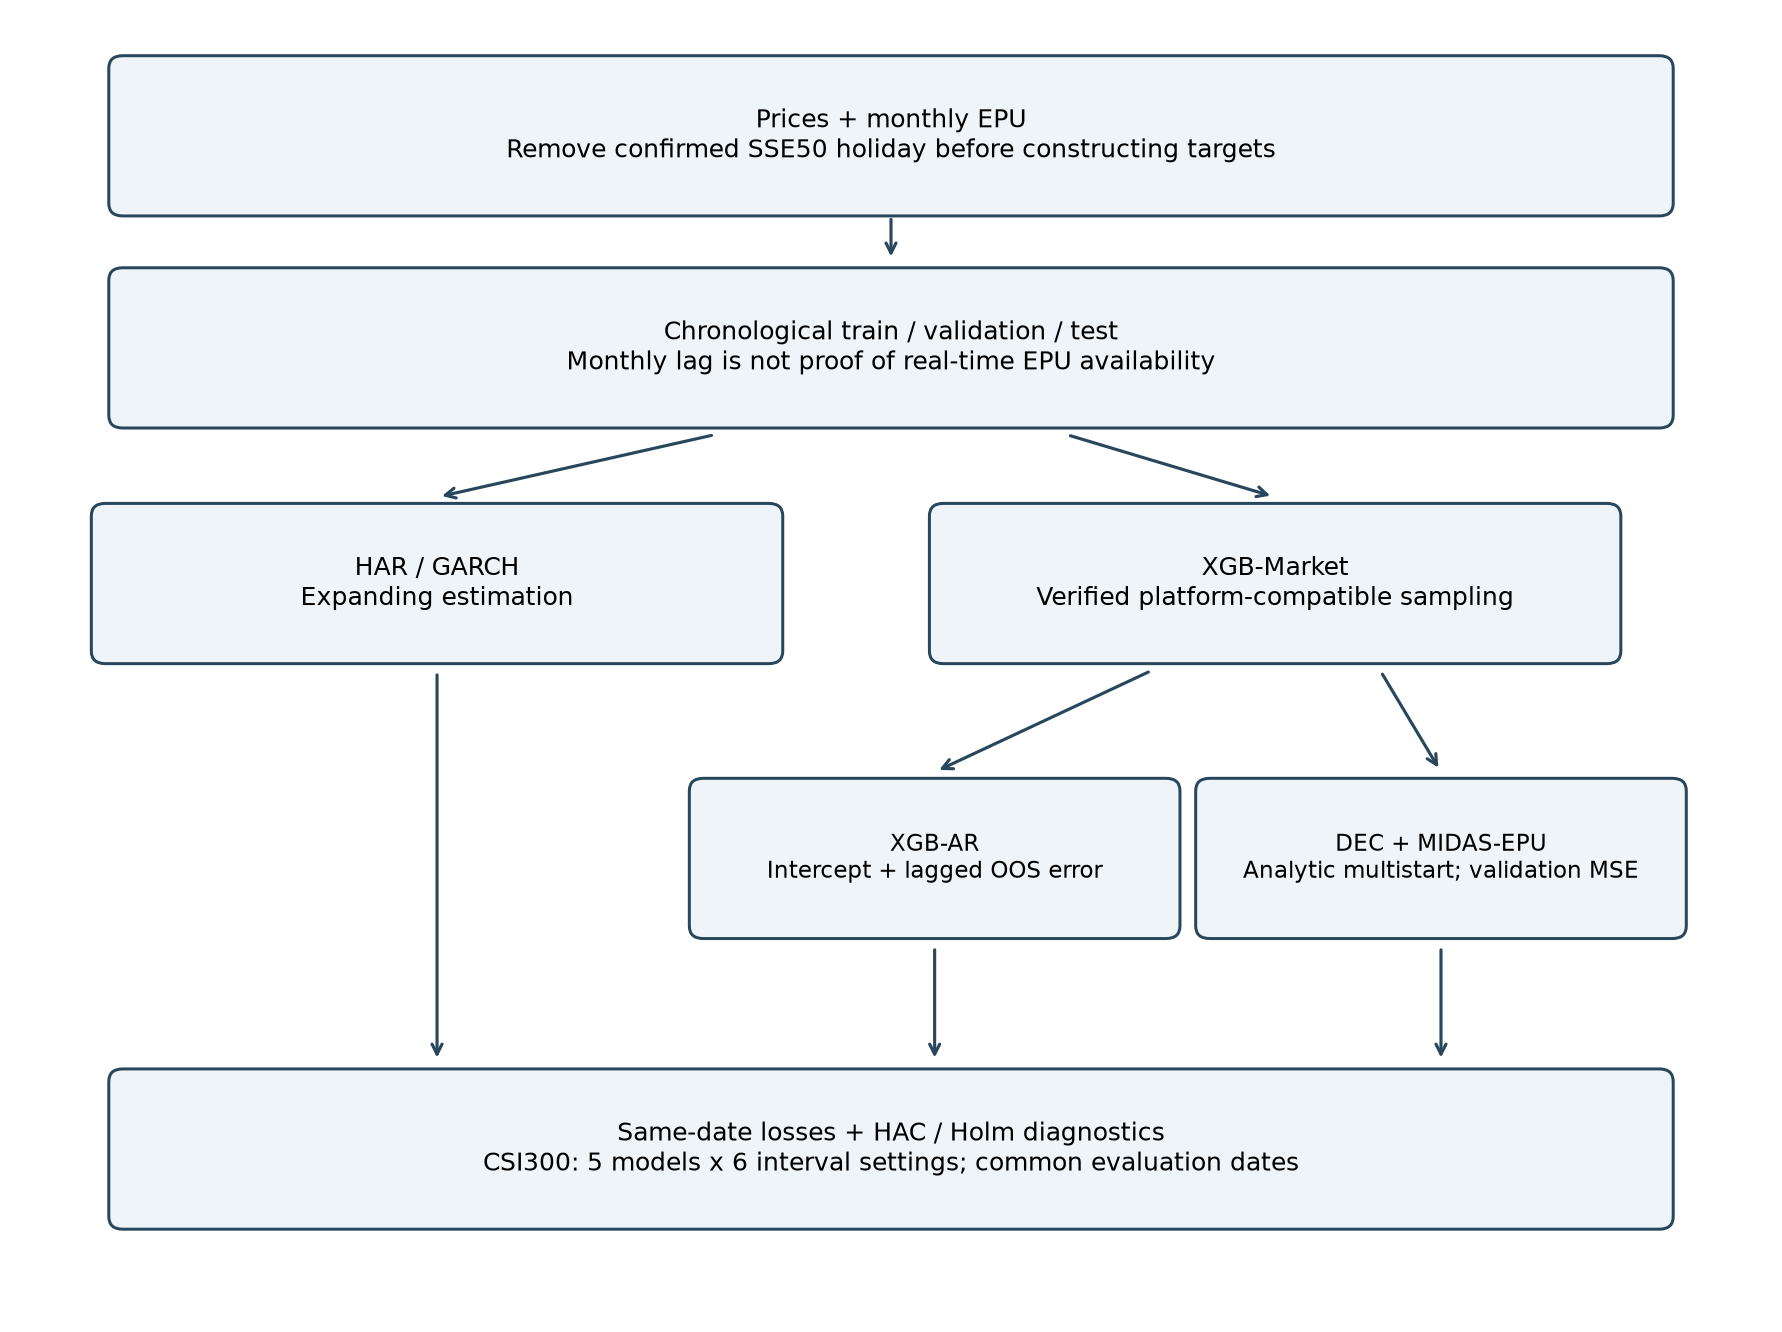
\includegraphics[width=1\textwidth]{../../results/revised/method_flow.png}
	\caption{修订研究流程：稳定求解、消融比较与共同日期评价}
	\label{fig:f}
\end{figure}


	
		
		
		
		
		
		
		
		
		
		
		
		
		
		
		
	


\subsection{本文组织结构}

本文共分为 5 章，具体安排如下：

第一章为绪论，主要介绍研究背景与意义、研究现状、研究内容与技术路线以及全文结构安排。

第二章为带动态误差修正机制的股指波动率预测模型，提出并详细推导了 XGB-MIDAS-EPU-DEC 混合预测模型，同时系统梳理了用于对比分析的各类基准模型。在此基础上，本章详细说明本文实证研究的数据来源与实验设计方案，并系统定义了点预测与区间预测的多维度评价指标体系，为后续的实证检验与结果分析奠定方法基础。

第三章为波动率点预测精度分析与结果检验，比较 XGB-MIDAS-EPU-DEC 模型和各类基准模型在 CSI 300 指数样本中的点预测表现，分析预测路径、损失函数结果、统计检验结果和 MIDAS-EPU 权重机制。

第四章为波动率区间预测精度分析与结果检验，基于滚动共形预测方法构造波动率预测区间，并从经验覆盖率、平均区间宽度、区间得分和覆盖检验等角度评价不同模型的区间预测表现。

第五章为 XGB-MIDAS-EPU-DEC 模型在其他样本下的稳健性分析，以上证 50 指数和纳斯达克综合指数作为替代样本，在相同实验框架下重复主要模型比较，以检验本文结论是否具有跨指数稳健性。
\section{理论基础与带动态误差修正机制的股指波动率预测模型}

本节介绍本文实证分析所使用的主要模型、预测设计与评价指标。本节在统一评价框架中考察点预测与区间预测的不同表现。为此，本文提出一种基于 XGBoost 框架的二段式误差修正模型 XGB-MIDAS-EPU-DEC，该模型通过 MIDAS 方法融合月度经济政策不确定性（EPU）数据，实现对基础模型预测误差的动态修正。本节首先系统梳理各类预测模型的数理基础，随后介绍了所采用的评价指标与方法。最后，本节将对样本划分和评价标准进行阐述。

\subsection{预测目标与基本符号}

设 \(C_t\) 表示第 \(t\) 个交易日的收盘价，日对数收益率 $r_t$ 定义为
\begin{equation}
	r_t=\ln\left(\frac{C_t}{C_{t-1}}\right).
\end{equation}
由于本文使用日度数据，无法直接基于高频日内收益率构造已实现波动率（realized volatility），因此采用日度平方收益率作为波动率代理变量：
\begin{equation}
	RV_t=r_t^2.
\end{equation}
为降低平方收益率分布偏态和极端值影响，并避免对零取对数，本文将一步超前对数波动率 $y_{t+1}$ 定义为主要预测目标：
\begin{equation}
	y_{t+1}=\ln(RV_{t+1}+\varepsilon),
	\qquad \varepsilon=10^{-8}.
\end{equation}
其中，\(\varepsilon\) 为极小正数。除特别说明外，本文所有点预测模型均以 \(y_{t+1}\) 为预测对象。对于需要在原始波动率尺度计算的指标，本文将对数预测值反变换为
\begin{equation}
	\widehat{RV}_{t+1|t}
	=
	\max\left\{
	\exp(\hat{y}_{t+1|t})-\varepsilon,\,
	10^{-12}
	\right\}.
\end{equation}

\paragraph{预测对象与反变换的限制}
平方收益率是条件二阶矩的噪声代理；仅在条件均值为零时，其条件期望等于条件方差。对数MSE训练趋向于条件对数均值，而指数反变换并不等于方差条件均值（Jensen不等式）。GARCH则直接预测条件方差。因而不同模型在MSE与QLIKE下的排序差异，部分可能来自预测目标和反变换差异，不能全部解释为算法优劣。区间覆盖对象是未来平方收益率的对数代理，而不是不可观测条件方差本身。\par

\subsection{基准模型}

金融资产收益率序列通常具有尖峰厚尾、波动聚集和条件异方差等典型特征。相应地，波动率预测模型需要能够刻画波动率的持续性、历史冲击影响以及条件方差动态。本文选取类 HAR 日度波动率模型和 GARCH(1,1) 模型作为传统基准模型，分别对应多尺度波动持续性和条件异方差递推机制。

\subsubsection{类 HAR 模型}

Corsi 提出的 HAR-RV 模型通过日度、周度和月度三个波动率成分近似刻画波动率的长期记忆特征，是波动率预测研究中的经典基准模型 \citep{Corsi2009}。原始 HAR-RV 模型通常基于高频数据构造已实现波动率。考虑到本文使用日度数据，本文借鉴 HAR 的多尺度思想，以平方收益率 \(RV_t=r_t^2\) 作为日度波动率代理。

定义过去 5 日和 22 日平均波动率分别为
\begin{equation}
	\overline{RV}_{t,5}
	=
	\frac{1}{5}\sum_{j=0}^{4}RV_{t-j},
	\qquad
	\overline{RV}_{t,22}
	=
	\frac{1}{22}\sum_{j=0}^{21}RV_{t-j}.
\end{equation}
则本文使用的类 HAR 日度波动率模型设定为
\begin{equation}
	y_{t+1}
	=
	\beta_0
	+
	\beta_d \ln(RV_t+\varepsilon)
	+
	\beta_w \ln(\overline{RV}_{t,5}+\varepsilon)
	+
	\beta_m \ln(\overline{RV}_{t,22}+\varepsilon)
	+
	u_{t+1}.
\end{equation}
其中，日度、周度和月度波动率成分分别刻画短期冲击、中短期波动背景和中期波动状态。该模型结构简单、解释明确，因此适合作为本文的线性波动率预测基准。

\subsubsection{GARCH(1,1) 模型}

Engle 提出的 ARCH 模型首次将条件方差建模为历史冲击平方的函数，Bollerslev 进一步提出 GARCH 模型，使条件方差同时依赖历史冲击和历史条件方差 \citep{Engle1982,Bollerslev1986}。GARCH(1,1) 模型通过递推结构刻画金融收益率中的波动聚集现象，是条件异方差建模中最常用的基准形式之一。

与现存代码一致，本文采用零条件均值及标准化 Student-t 扰动设定，均值和方差方程为：
\begin{equation}
	r_t=\epsilon_t,
	\qquad
	\epsilon_t=\sqrt{h_t}z_t,
\end{equation}
其中 \(h_t\) 为条件方差，\(z_t\) 为均值为 0、方差为 1 的标准化扰动项。GARCH(1,1) 条件方差方程为
\begin{equation}
	h_t
	=
	\omega
	+
	\alpha \epsilon_{t-1}^{2}
	+
	\beta h_{t-1},
	\qquad
	\omega>0,\quad \alpha\geq0,\quad \beta\geq0.
\end{equation}
在标准GARCH假设下，为获得有限的无条件二阶矩，通常要求
\begin{equation}
	\alpha+\beta<1.
\end{equation}
在一步超前预测中，若 \(E(z_t^2)=1\)，则
\begin{equation}
	E(r_{t+1}^{2}\mid \mathcal{F}_t)=h_{t+1}.
\end{equation}
因此，GARCH(1,1) 的一步超前对数波动率预测 $\hat{y}^{GARCH}_{t+1|t}$ 定义为
\begin{equation}
	\hat{y}^{GARCH}_{t+1|t}
	=
	\ln(\hat{h}_{t+1|t}+\varepsilon).
\end{equation}
本文不进一步引入 EGARCH、GJR-GARCH 等扩展模型，原因在于本文目标不是穷尽 GARCH 模型族，而是在统一预测框架下比较传统强基准、机器学习基准和本文提出的两阶段修正模型。

\subsection{基于 MIDAS-EPU 动态误差修正的 XGBoost 波动率预测模型}

本文提出基于 MIDAS-EPU 动态误差修正的 XGBoost 波动率预测模型，即 XGBoost Volatility Forecasting Model with MIDAS-EPU Dynamic Error Correction，简称 XGB-MIDAS-EPU-DEC。该模型采用两阶段结构：第一阶段首先使用日度市场变量构建 XGB-Market 机器学习基准预测，随后在第二阶段利用历史样本外预测残差和 MIDAS 加权的月度经济政策不确定性信息构造动态误差修正项。最终预测由第一阶段基准预测与第二阶段误差修正项相加得到。

\subsubsection{XGB-Market 基准模型}

XGBoost 是一种基于梯度提升树的集成学习方法，能够通过逐步叠加回归树逼近复杂非线性函数，并在目标函数中加入正则化项以控制模型复杂度 \citep{ChenGuestrin2016}。与线性模型相比，XGBoost 能够更灵活地刻画变量之间的非线性关系和交互效应，因此适合用于包含多类市场特征的波动率预测任务。

设 \(X_t^M\) 表示第 \(t\) 个交易日可观测的日度市场特征向量，包括历史波动率、收益率、价格振幅和成交量等变量。第一阶段 XGB-Market 模型可表示为
\begin{equation}
	\hat{y}^{XGB}_{t+1|t}
	=
	f_{XGB}(X_t^M),
\end{equation}
其中 \(f_{XGB}(\cdot)\) 表示由训练样本估计得到的非线性映射函数。本文将 XGB-Market 作为机器学习基准模型，用于检验仅依赖日度市场变量的非线性模型是否能够提供样本外预测增益。

\subsubsection{MIDAS-EPU 变量构造}

本文使用的经济政策不确定性指数为月度频率，而股指市场变量为日度频率，因此二者构成混频数据结构。若直接将月度 EPU 简单填充至日度样本，难以刻画低频变量的滞后影响；若直接纳入多个滞后月份变量，则可能造成参数过多和样本效率下降。MIDAS 方法通过参数化权重函数将低频变量的多期滞后压缩为少量参数，适用于处理不同频率变量之间的预测关系 \citep{GhyselsSinkoValkanov2007,EngleGhyselsSohn2013}。

设交易日 \(t\) 所属自然月份为 \(m(t)\)。现存代码不使用当月 EPU，而按月份标签使用 \(m(t)-1\) 及更早月份的信息。月份滞后并不能证明实际发布日期之前可得；未保存逐日发布日与历史修订版本，因此这里只能称为回顾性伪样本外实验。给定滞后长度 \(K\)，MIDAS-EPU 指标 $\widetilde{EPU}_{t}^{(K,\boldsymbol{\theta})}$ 定义为
\begin{equation}
	\widetilde{EPU}_{t}^{(K,\boldsymbol{\theta})}
	=
	\sum_{k=1}^{K}
	w(k;\boldsymbol{\theta})
	\ln(EPU_{m(t)-k}),
\end{equation}
其中 \(w(k;\boldsymbol{\theta})\) 为权重函数，并满足
\begin{equation}
	w(k;\boldsymbol{\theta})\geq0,
	\qquad
	\sum_{k=1}^{K}w(k;\boldsymbol{\theta})=1.
\end{equation}
本文主要考虑 Beta 权重和指数 Almon 权重两类常见 MIDAS 权重函数。Beta 权重定义为
\begin{equation}
	w^{B}(k;\theta_1,\theta_2)
	=
	\frac{a_k}{\sum_{j=1}^{K}a_j},
    \quad a_k=\max\{x_k^{\theta_1-1}(1-x_k)^{\theta_2-1},10^{-12}\},
	\qquad
	x_k=\frac{K-k+1}{K+1}.
\end{equation}
为与保存的权重及参数一致，令 $z_k=(K-k+1)/K$，指数 Almon 权重定义为
\begin{equation}
	w^{EA}(k;\theta_1,\theta_2)
	=
	\frac{
		\exp(\theta_1 z_k+\theta_2 z_k^2)
	}{
		\sum_{j=1}^{K}\exp(\theta_1 z_j+\theta_2 z_j^2)
	}.
\end{equation}

\subsubsection{XGB-MIDAS-EPU-DEC 动态误差修正模型}

第一阶段 XGB-Market 模型生成基准预测值后，本文进一步构造其样本外预测残差。设第一阶段模型在时点 \(t-1\) 对 \(y_t\) 的预测为 \(\hat{y}^{XGB}_{t|t-1}\)，则样本外残差 $e_t$ 定义为
\begin{equation}
	e_t
	=
	y_t-\hat{y}^{XGB}_{t|t-1}.
\end{equation}
其中 \(e_t\) 必须是真实样本外残差，而不是样本内拟合残差。若使用样本内残差训练第二阶段模型，可能会将第一阶段模型的过拟合误差误认为可利用的动态结构，从而高估模型的预测能力。

第二阶段误差修正模型设定 $e_{t+1}$ 为
\begin{equation}
	e_{t+1}
	=
	\alpha_0
	+
	\rho e_t
	+
	\gamma
	\widetilde{EPU}_{t}^{(K,\boldsymbol{\theta})}
	+
	u_{t+1}.
	\label{eq:error_correction}  
\end{equation}
式 \eqref{eq:error_correction} 本质上是一个 ARX(1) 回归模型，用于预测 $e_{t+1}$。其中，\(e_t\) 反映预测误差的短期持续性，\(\widetilde{EPU}_{t}^{(K,\boldsymbol{\theta})}\) 表征低频政策不确定性与预测偏差的滞后关联。最终预测值 $\hat{y}^{final}_{t+1|t}$ 为
\begin{equation}  
	\hat{y}^{final}_{t+1|t}
	=
	\hat{y}^{XGB}_{t+1|t}
	+
	\hat{e}_{t+1|t}.
\end{equation}

该框架的主要特点是将“日度市场变量的非线性预测能力”和“月度政策不确定性的误差修正作用”分层建模。第一阶段负责提取市场变量中的非线性信息，第二阶段检验历史残差与EPU组合的预测表现，不能仅凭该组合识别EPU单独贡献。需要注意的是，第二阶段中的残差 \(e_t\) 属于生成回归量，相关系数不宜解释为严格因果效应 \citep{Pagan1984}。因此，本文关注的是该修正机制能否改善样本外预测表现，而非识别 EPU 对股指波动率的结构性因果效应。

\paragraph{第二阶段的修订估计与规格选择}
给定窗口$K$、权重族及形状参数$\theta$，线性系数通过OLS估计。将剖面目标写为
\[
 F(\theta)=n^{-1}\min_{a,\rho,\gamma}\|e-a\mathbf1-\rho e_{-1}-\gamma Lw(\theta)\|^2.
\]
其中$L$为训练段月度对数EPU滞后矩阵。通过SVD将$e$及$L$投影到截距和滞后残差的正交补，消去线性控制项；这种变量投影思路用于可分离非线性最小二乘\citep{GolubPereyra1973}。设最优线性回归残差为$r$，在秩不变且权重可微处，剖面梯度为
\[
 \nabla_\theta F=-\frac{2\hat\gamma}{n}\left(L\frac{\partial w}{\partial\theta}\right)^\top r.
\]
Beta仍保留归一化前$10^{-12}$下截；低于阈值的原始权重导数设为零，阈值处为分段可微。本文没有改变权重族或参数范围来追求测试指标。

旧版使用单起点L-BFGS-B、前向差分及默认相对目标停止阈值；部分成功标志没有对应足够小的梯度，且可能停在不同局部解。修订版最小化平均平方残差并传入解析梯度。Beta两参数范围均为$[0.05,20]$，采用$\{0.05,0.5,1.5,5,20\}\times\{0.05,0.5,2,5,20\}$的25个起点；指数Almon范围均为$[-5,5]$，采用$\{-5,-2.5,0,2.5,5\}^2$及旧起点$(-0.2,-0.02)$，共26个起点。L-BFGS-B的$ftol=10^{-14}$、$gtol=10^{-9}$、最大迭代2000、最大函数调用10000、最大线搜索50。投影梯度超过$10^{-6}$时从该候选点用SLSQP重试。每次选择训练目标最低的候选；若该解仍不满足$10^{-6}$验收阈值则报错，不据测试表现替换解。停止规则的区别见SciPy官方说明\footnote{\url{https://docs.scipy.org/doc/scipy/reference/optimize.minimize-lbfgsb.html}}。

第一阶段顺序生成500条验证样本的样本外预测。构造一阶残差滞后后，499条有效残差按时间分为299条估计与200条评分。对$K\in\{6,12,24\}$及两种权重族共六组规格，按后200条残差预测MSE选取；评分段使用已实现的前期残差，参数不重估。测试期固定窗口和权重族，每60条保留观测重新估计形状参数及线性系数，训练只包含此前已经实现的样本外残差。求解规则在本轮新测试结果产生前固定，但历史结果已被查看，故本轮属于回顾性方法修订，不是预注册验证。

\paragraph{残差单独修正的消融对照}
新增XGB-AR：$\hat y^{AR}_{t+1|t}=\hat y^{XGB}_{t+1|t}+\hat a+\hat\rho e_t$。它不含EPU，使用与DEC相同的可用历史残差、扩展窗口及60条重估间隔，以OLS估计，没有新增调参。DEC与XGB-AR的比较用于评价该设定下加入EPU的增量表现；它仍不能识别外生政策冲击、排除数据版本问题或建立因果关系。

\subsection{研究假设}

基于上述理论机制与模型设定，本文并不预设复杂模型必然优于传统模型，而是在统一的样本外预测框架下检验不同信息来源和模型结构是否具有增量预测价值。具体而言，本文遵循以下研究假设。

\textbf{假设 H1：股指波动率具有持续性与多尺度依赖结构。}

金融资产收益率通常存在波动聚集和条件异方差特征，意味着高波动状态往往会在短期内延续，低波动状态也具有一定持续性。同时，不同期限投资者的信息处理周期和交易行为存在差异，使得未来波动率可能同时受到日度、周度和月度历史波动状态的影响。因此，本文预期基于历史波动率构造的 HAR 类变量能够为下一期波动率预测提供有效信息。

\textbf{假设 H2：日度市场变量中存在可由非线性模型捕捉的预测信息。}

传统线性模型虽然具有较强解释性，但其对变量间非线性关系和交互效应的刻画能力有限。股指波动率可能同时受到历史波动、收益率冲击、价格振幅和成交量变化等多类市场变量影响，且这些变量之间的关系未必满足简单线性形式。因此，本文预期 XGB-Market 模型能够从日度市场变量中提取一定非线性预测信息，但其样本外表现仍需与 HAR 和 GARCH 等传统强基准进行比较。

\textbf{假设 H3：经济政策不确定性包含股指波动率预测的增量信息。}

经济政策不确定性可能通过影响投资者预期、风险补偿要求、市场流动性和交易行为等渠道改变股票市场风险状态。由于政策信息从形成、传播到被市场吸收通常存在一定时滞，EPU 对股指波动率的影响未必表现为即时冲击，而可能具有滞后性和持续性。因此，本文预期经过 MIDAS 权重重构的 EPU 信息能够解释第一阶段市场模型未能捕捉的部分系统性预测误差。

\textbf{假设 H4：动态误差修正能够改善单一机器学习模型的样本外预测表现。}

如果 XGB-Market 的样本外预测残差并非纯随机噪声，而是仍包含残差持续性或低频政策不确定性信息，则在第一阶段预测基础上引入动态误差修正项应当能够改善最终预测结果。基于此，本文预期 XGB-MIDAS-EPU-DEC 模型相对于单一 XGB-Market 模型具有一定增量预测价值，并可能在点预测精度与区间预测表现之间取得相对平衡。

本轮用XGB-AR进行EPU消融比较，但H3的判断仍须区分损失函数和市场，不能把局部指标改善解释为全面预测优势。需要说明的是，上述假设均属于预测意义上的经验假设，而非严格因果识别命题。本文关注的是不同变量和模型结构是否能够在样本外预测中提供有效增量信息，而不将 EPU 系数或误差修正项解释为政策不确定性对股指波动率的结构性因果效应。

\subsection{XGB-Market 模型变量构造}

被解释变量的设定与前文相同，即核心预测对象为下一交易日对数波动率。

解释变量主要由日度市场变量构造，包括三类。第一类为多尺度历史波动率变量，用于刻画波动率持续性：
\begin{equation}
	\ln RV_t=\ln(RV_t+\varepsilon),
\end{equation}
\begin{equation}
	\ln \overline{RV}_{t,5}
	=
	\ln\left(\frac{1}{5}\sum_{i=0}^{4}RV_{t-i}+\varepsilon\right),
\end{equation}
\begin{equation}
	\ln \overline{RV}_{t,22}
	=
	\ln\left(\frac{1}{22}\sum_{i=0}^{21}RV_{t-i}+\varepsilon\right).
\end{equation}
第二类为收益率方向变量：
\begin{equation}
	r_t^{+}=\max(r_t,0),\qquad
	r_t^{-}=\min(r_t,0).
\end{equation}
第三类为价格振幅和成交量变量。设 \(H_t\)、\(L_t\)、\(V_t\) 分别表示第 \(t\) 个交易日最高价、最低价和成交量，则日内振幅 $R_t$ 定义为
\begin{equation}
	R_t=\ln\left(\frac{H_t}{L_t}\right),
\end{equation}
短期振幅均值 $\overline{R}_{t,5}$ 定义为
\begin{equation}
	\overline{R}_{t,5}
	=
	\frac{1}{5}\sum_{i=0}^{4}R_{t-i}.
\end{equation}
成交量变量包括对数成交量水平和对数成交量变化率：
\begin{equation}
	\ln V_t,\qquad
	\Delta \ln V_t=\ln V_t-\ln V_{t-1}.
\end{equation}

表 \ref{tab:variables_main} 汇总了本文主要变量定义。

\begin{table}[!htbp]
	\centering
	\makebox[\textwidth][c]{
		\begin{threeparttable}
			\captionsetup{font=small,skip=3pt}
			\caption{主要市场变量定义}
			\label{tab:variables_main}
			
			\begingroup
			\footnotesize
			\setlength{\tabcolsep}{4pt}
			\renewcommand{\arraystretch}{1.13}
			
			\begin{tabularx}{0.90\textwidth}{
					>{\raggedright\arraybackslash}p{2.55cm}
					>{\centering\arraybackslash}p{2.35cm}
					>{\centering\arraybackslash}X
				}
				\toprule
				变量名称 & 符号 & 数学定义 \\
				\midrule
				日对数收益率 & \(r_t\) & \(\ln(C_t/C_{t-1})\) \\
				波动率代理变量 & \(RV_t\) & \(r_t^2\) \\
				一步超前预测目标 & \(y_{t+1}\) & \(\ln(RV_{t+1}+\varepsilon)\) \\
				即时历史波动率 & \(\ln RV_t\) & \(\ln(RV_t+\varepsilon)\) \\
				周度历史波动率 & \(\ln \overline{RV}_{t,5}\) & \(\ln\{5^{-1}\sum_{i=0}^{4}RV_{t-i}+\varepsilon\}\) \\
				月度历史波动率 & \(\ln \overline{RV}_{t,22}\) & \(\ln\{22^{-1}\sum_{i=0}^{21}RV_{t-i}+\varepsilon\}\) \\
				正收益项 & \(r_t^+\) & \(\max(r_t,0)\) \\
				负收益项 & \(r_t^-\) & \(\min(r_t,0)\) \\
				日内振幅 & \(R_t\) & \(\ln(H_t/L_t)\) \\
				短期振幅均值 & \(\overline{R}_{t,5}\) & \(5^{-1}\sum_{i=0}^{4}R_{t-i}\) \\
				成交量水平 & \(\ln V_t\) & \(\ln(V_t)\) \\
				成交量变化率 & \(\Delta\ln V_t\) & \(\ln(V_t)-\ln(V_{t-1})\) \\
				\bottomrule
			\end{tabularx}
			\endgroup
			
			\begin{tablenotes}[flushleft]
				\scriptsize
				\item 注：\(C_t\)、\(H_t\)、\(L_t\) 和 \(V_t\) 分别表示第 \(t\) 个交易日的收盘价、最高价、最低价和成交量；\(\varepsilon=10^{-8}\)，用于避免对零取对数。除一步超前预测目标 \(y_{t+1}\) 外，表中解释变量均为 \(t\) 时点及以前可观测的市场变量，用于第一阶段 XGB-Market 预测模型。EPU 信息不作为本表中的市场解释变量，而是在第二阶段通过 MIDAS-EPU 因子进入动态误差修正模型。
			\end{tablenotes}
		\end{threeparttable}
	}
\end{table}


由于部分解释变量依赖过去 5 个或 22 个交易日的信息，滚动计算会导致样本前段产生不可定义观测；同时，主预测目标 \(y_{t+1}\) 需要使用下一交易日收益率，因此样本末端也会自然损失少量观测。本文在建模前统一删除由变量构造导致的缺失观测。此类处理并非对原始数据进行插补或平滑，而是由预测变量定义和超前目标构造自然决定。

本文的核心任务是预测股指下一交易日对数波动率，并在统一的伪样本外框架下比较传统波动率模型、机器学习基准模型以及本文提出的 XGB-MIDAS-EPU-DEC 模型。为避免不同章节之间重复，本节不再展开数据来源和具体变量清洗过程，而是重点说明模型设定、预测目标、样本外预测原则以及点预测和区间预测的评价方法。

\subsection{数据来源与样本处理}

本文使用CSI300日度行情，字段包括日期、开高低收与成交量，范围为2010年1月至2026年3月。现存输入有3942条价格，按相邻收盘价比值计算并删除首个不可定义值后，得到3941条收益率。公开版的描述统计、检验及相应图件均据此重新生成。历史3942条统计可由在2018年6月15日与6月19日收益率之间额外插入一个零值精确重构，包括10项描述统计及JB、Ljung--Box、ARCH检验，共24个数值；插入操作仅用于追查，未作为真实数据使用。额外记录的原始日期及形成过程没有保存，不能认定为某个交易日或首行填充值。

三个指数的日期、全部市场特征、24个月EPU滞后及训练/验证/测试划分均可由现存输入重建，与保存的建模矩阵在数值容差内一致。CSI300建模矩阵为3919行，未包含上述额外零值；描述统计差异不能据此归结为最终预测输入错配。

经济政策不确定性变量采用 Davis、Liu 和 Sheng 基于中国大陆报纸构造的中国经济政策不确定性指数（China Economic Policy Uncertainty Index, China EPU）月度数据 \citep{DavisLiuSheng2019}。由于市场数据为日度频率，而 EPU 数据为月度频率，代码以月度滞后对齐EPU；没有原始发布日与修订版本，不能独立证明实时可得性。行情预测原点为交易日收盘后。

\subsection{数据统计学特征检验}

为确认主样本是否具有典型金融时间序列特征，本文对 CSI 300 日对数收益率进行描述性统计、正态性检验、自相关检验和条件异方差检验。表 \ref{tab:desc_return_short} 汇报了日对数收益率的主要描述性统计结果。

\begin{table}[!htbp]
	\centering
	\caption{CSI 300 日对数收益率描述性统计（3941条收益率，已复算）}
	\label{tab:desc_return_short}
	\begingroup
	\footnotesize
	\setlength{\tabcolsep}{5pt}
	\renewcommand{\arraystretch}{1.08}
	\begin{tabular}{lcccccc}
		\toprule
		样本量 & 均值 & 标准差 & 最小值 & 最大值 & 偏度 & 超额峰度 \\
		\midrule
		3941 & \(5.8396\times10^{-5}\) & 0.013639 & -0.091544 & 0.081420 & -0.576130 & 5.460548 \\
		\bottomrule
	\end{tabular}
	\endgroup
\end{table}

结果显示，CSI 300 日对数收益率均值接近零，标准差为 0.013639；收益率分布存在左偏，样本超额峰度大于零，说明样本具有尖峰厚尾特征。如图 \ref{fig:return_ts_qq}，提供了尖峰厚尾特征的图像证据。为进一步检验收益率序列的分布和动态依赖性质，本文报告 Jarque--Bera 检验、Ljung--Box 检验和 ARCH-LM 检验结果，如表 \ref{tab:diagnostic_tests_short} 所示。

\begin{table}[!htbp]
	\centering
	\caption{CSI 300 日对数收益率统计特征检验（3941条收益率，已复算）}
	\label{tab:diagnostic_tests_short}
	\footnotesize
	\setlength{\tabcolsep}{6pt} 
	\renewcommand{\arraystretch}{1.08}
	\begin{tabular}{l c c r} 
		\toprule
		检验 & 对象/滞后阶数 & 统计量 & \(p\)-value \\
		\midrule
		Jarque--Bera & \(r_t\) & 5099.01 & $<0.0001$ \\
		Ljung--Box & \(r_t\), 10阶 & 32.75 & 0.0003 \\
		Ljung--Box & \(r_t\), 20阶 & 64.45 & \(1.43\times10^{-6}\) \\
		Ljung--Box & \(r_t^2\), 10阶 & 1051.71 & \(1.35\times10^{-219}\) \\
		Ljung--Box & \(r_t^2\), 20阶 & 1526.13 & \(9.87\times10^{-312}\) \\
		ARCH-LM & 10阶 & 452.36 & \(6.56\times10^{-91}\) \\
		ARCH-F & 10阶 & 50.98 & \(9.52\times10^{-97}\) \\
		\bottomrule
	\end{tabular}
\end{table}

\begin{figure}[H]
	\centering 
	\subfigure[CSI 300 日对数收益率时序图]{ 
		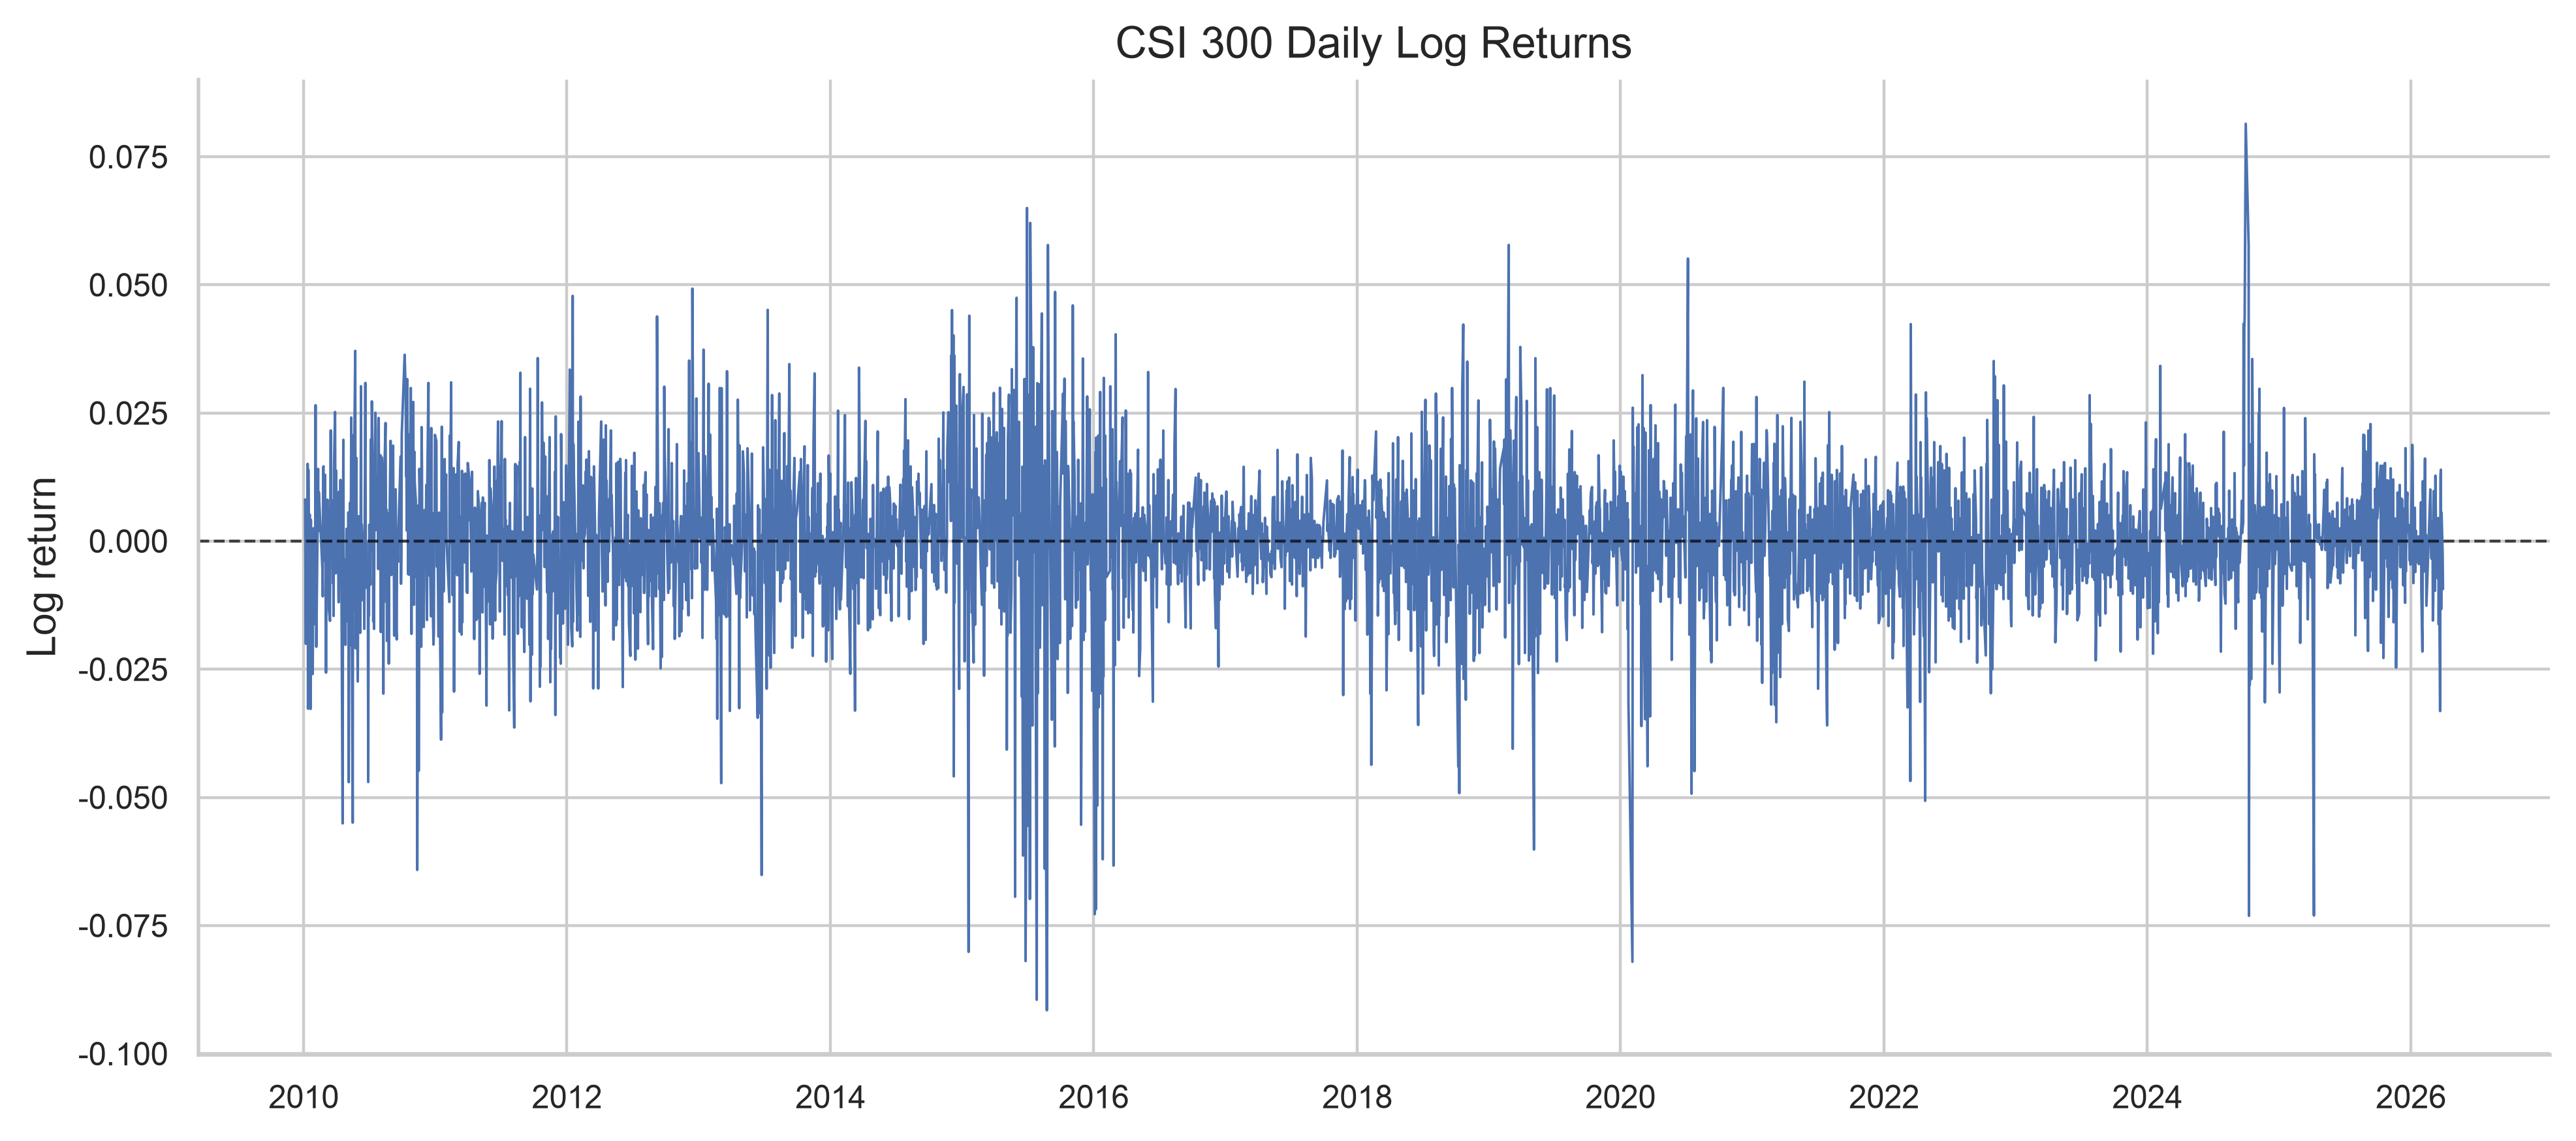
\includegraphics[width=0.47\textwidth]{../../results/descriptive-corrected/figure_1_log_return_series.png} } 
	\hfill 
	\subfigure[CSI 300 日对数收益率 QQ 图]{ 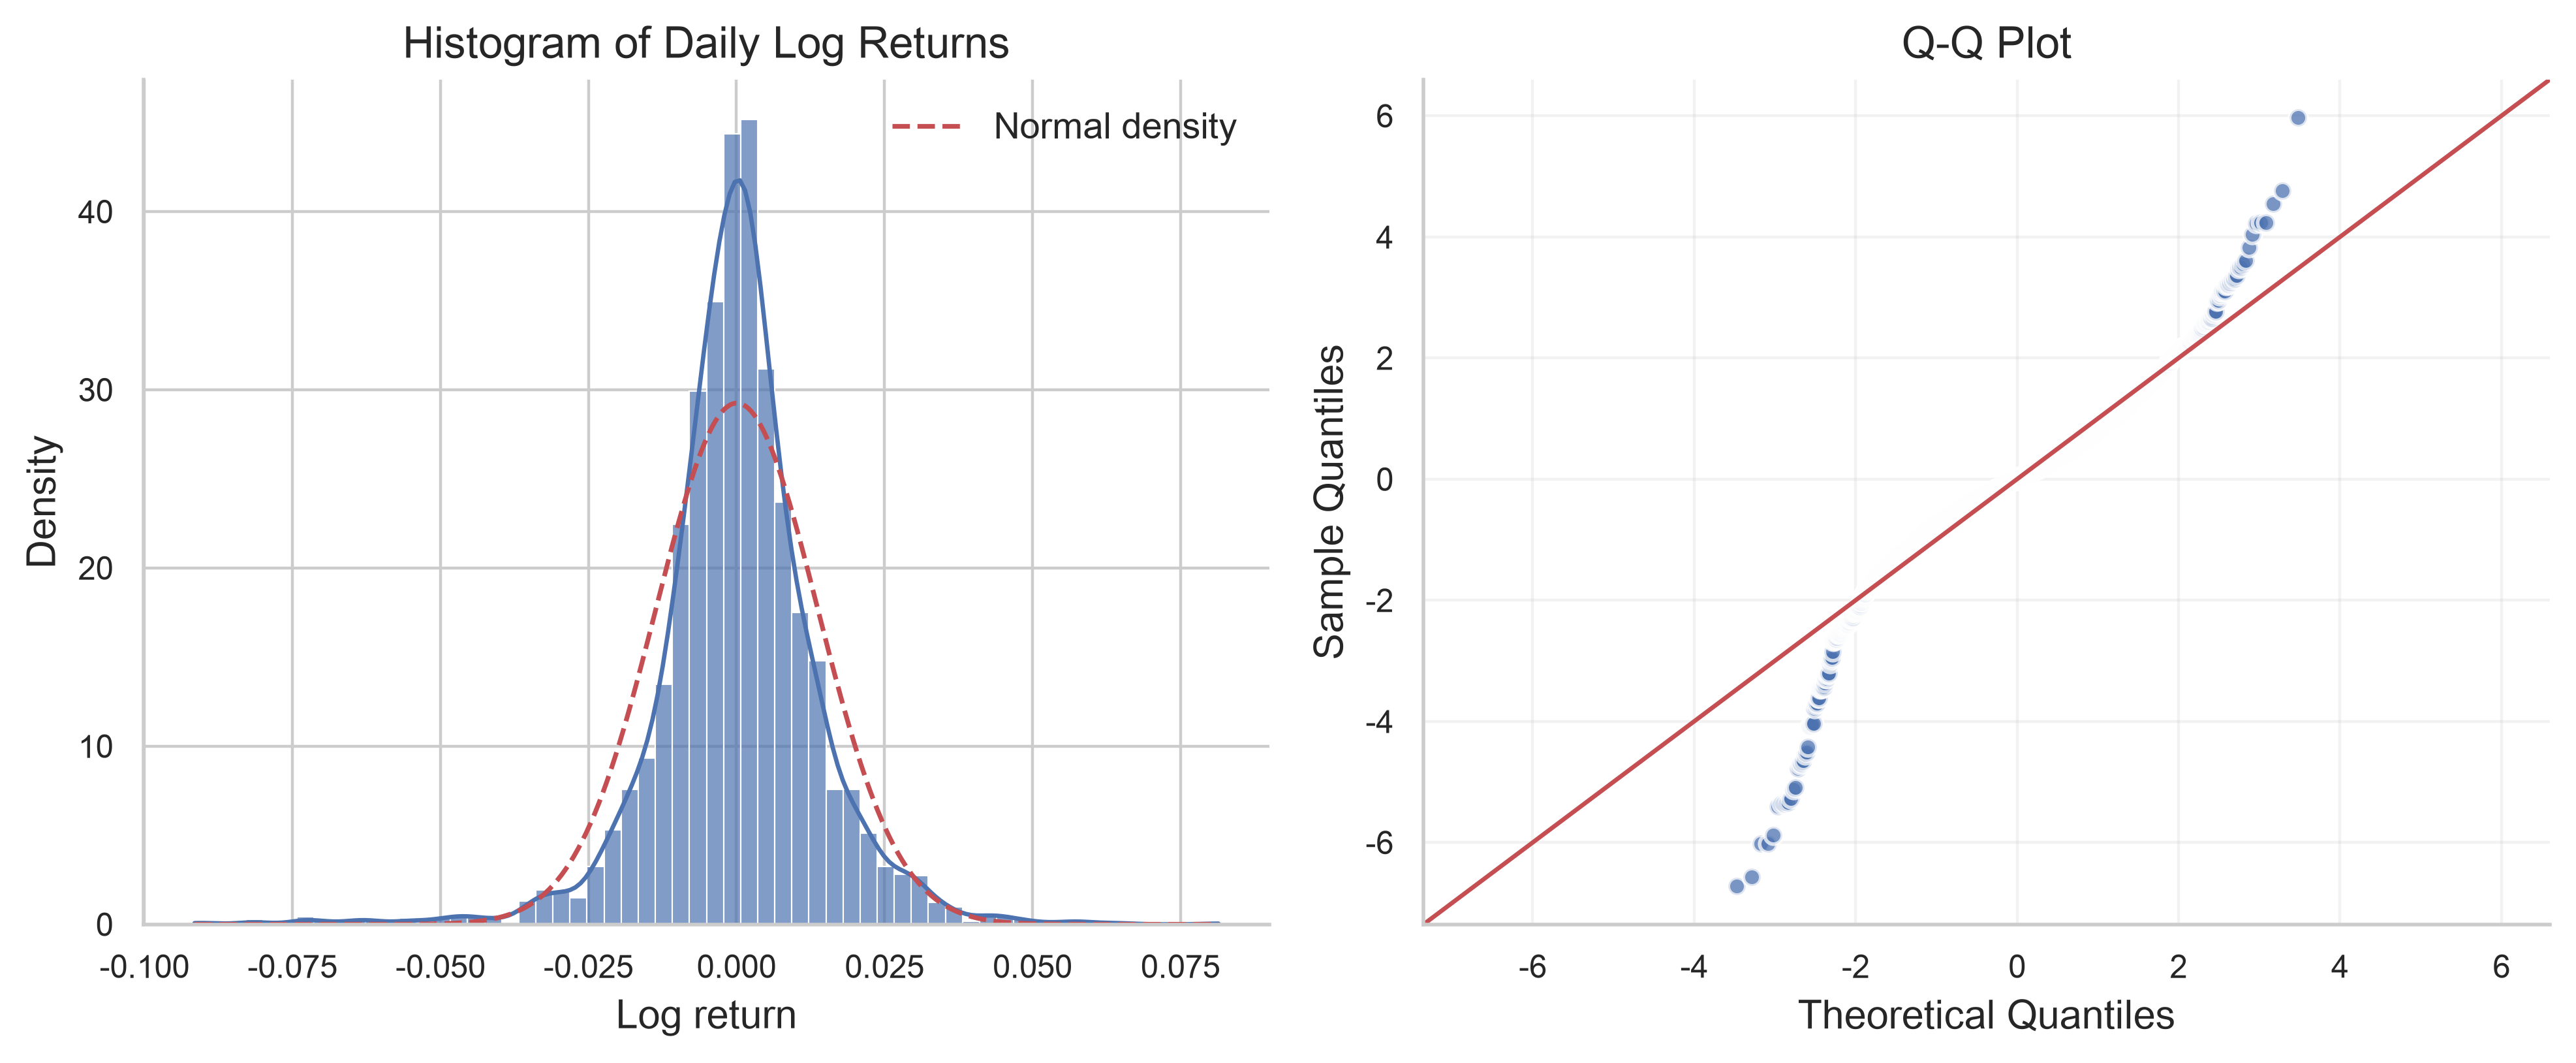
\includegraphics[width=0.47\textwidth]{../../results/descriptive-corrected/figure_2_histogram_qq.png} } 
	\caption{CSI 300 日对数收益率序列图形特征} 
	\label{fig:return_ts_qq} 
\end{figure}

Jarque--Bera 检验拒绝收益率正态分布假设；平方收益率的 Ljung--Box 检验在所报告滞后下拒绝无自相关原假设，提示波动率代理序列存在序列依赖；ARCH-LM 检验显著拒绝同方差假设，表明收益率序列具有条件异方差特征。上述结果为后续使用 HAR 类变量、GARCH 模型和非线性预测模型提供了经验依据。

\subsection{伪样本外预测设计}

在预测过程中，本文采用一步超前预测框架。设 \(\mathcal{F}_t\) 表示时点 \(t\) 已经可获得的信息集，则所有模型在预测 \(y_{t+1}\) 时只能使用 \(\mathcal{F}_t\) 中的信息：
\begin{equation}
	\hat{y}_{t+1|t}
	=
	g(\mathcal{F}_t).
\end{equation}
随着时间推进，训练窗口逐步向前扩展。对于 HAR 和 GARCH(1,1) 模型，本文在扩展窗口内递推估计模型参数并生成一步超前预测；对于 XGB-Market 模型，本文使用固定300轮、深度4等附录配置，在扩展窗口中每20条保留观测重训，不采用固定长度滚动窗口或早停；对于 XGB-MIDAS-EPU-DEC 模型，第二阶段误差修正层仅使用已经实现的历史样本外残差。

伪样本外预测设计的关键在于信息集闭合。尤其对于本文的两阶段模型，第二阶段误差修正不能使用尚未实现的残差。只有当 \(y_t\) 实现之后，残差
\begin{equation}
	e_t=y_t-\hat{y}_{t|t-1}
\end{equation}
才可以作为时点 \(t\) 之后的可用信息进入误差修正模型。该处理是避免前视偏差和样本内过拟合的重要条件。

\paragraph{代码行号、缺失行与交易日历限制}
代码中日期为 $t$ 的行保存的是超前目标 $y_{t+1}$；第一阶段重训使用该行之前的行，其最后一个目标在收盘时已经实现。第二阶段同样在预测原点前截断训练行。市场特征仅作本文所列对数、滚动均值和缺失处理，匹配存档的主流程没有缩尾、标准化或第一阶段内部早停。这里的20与60为过滤后行数，存在缺口时不应直接称为20或60个连续交易日。

此外，历史代码先在原价格行上计算收益率与超前目标，再删除缺失特征行；残差滞后则对保留行作一次位移。无缺口时它等于式\eqref{eq:error_correction}中的 $e_t$；有缺口时应理解为最近保留预测所对应、已经实现的残差，并不一定是紧邻交易日残差。上证50历史测试段的2018年6月25日存在一处这种情况；本轮先删除确认的休市行后该处缺口消失。其他零成交量及缺失特征仍需完整日历审计。

上证50源表还把2018年6月18日列为与前一行同收盘价、零成交量的记录，而上交所公告确认该日休市\footnote{上海证券交易所《关于上海证券交易所2018年全年休市安排的通知》，2017-12-22，公告〔2017〕26号，端午节安排。}。尽管该行的缺失成交量特征后来被删除，6月15日行的超前目标仍指向它，产生 $\ln(10^{-8})$ 的人工零收益目标，并影响相邻滚动特征。因此，“下一交易日”是研究设计目标，并非上证50历史数据所有行都满足的已验证事实。历史结果保留在归档目录；本文正文的修订上证50实验先排除该休市行，重建收益率、目标及特征，再生成全部基准和修正模型预测。修订样本为1500/500/1919，不能只删一条测试损失代替重估。附录另保留上一轮日历清洗对照。其他零成交量记录不凭此一项特征认定为休市。

\subsection{波动率点预测评价方法}

\subsubsection{MSE 与 MAE}

本文首先使用均方误差（Mean Squared Error, MSE）和平均绝对误差（Mean Absolute Error, MAE）评价模型在对数波动率代理尺度上的预测精度。设测试集共有 \(N\) 个预测观测，真实值为 \(y_{t+1}\)，预测值为 \(\hat{y}_{t+1|t}\)，则
\begin{equation}
	MSE
	=
	\frac{1}{N}
	\sum_{t=1}^{N}
	\left(
	y_{t+1}-\hat{y}_{t+1|t}
	\right)^2,
\end{equation}
\begin{equation}
	MAE
	=
	\frac{1}{N}
	\sum_{t=1}^{N}
	\left|
	y_{t+1}-\hat{y}_{t+1|t}
	\right|.
\end{equation}
MSE 对极端误差更敏感，MAE 则更直接反映平均绝对偏离。二者结合可以从不同角度评价模型在对数波动率代理尺度上的预测表现。

\subsubsection{QLIKE 损失函数}

由于真实条件方差无法直接观测，波动率预测通常需要借助代理变量进行评价。Patton 指出，在波动率代理变量存在测量误差时，损失函数的选择可能影响模型排序，QLIKE 损失函数在波动率预测评价中具有在代理条件无偏等前提下的排序稳健性 \citep{Patton2011}。因此，本文将 QLIKE 作为重要补充指标。

设真实波动率代理为 \(RV_{t+1}\)，模型预测方差为 \(\widehat{RV}_{t+1|t}\)，则 QLIKE 定义为
\begin{equation}
	QLIKE
	=
	\frac{1}{N}
	\sum_{t=1}^{N}
	\left[
	\frac{RV_{t+1}}{\widehat{RV}_{t+1|t}}
	-
	\ln
	\left(
	\frac{RV_{t+1}}{\widehat{RV}_{t+1|t}}
	\right)
	-
	1
	\right].
\end{equation}
QLIKE 值越低，表示模型在原始方差尺度上的预测表现越好。实现时，观测代理与预测值在对数反变换后均下截至 $10^{-12}$，再计算比值及其对数；这避免零值导致未定义损失，但属于数值截断，不保证截断后的代理仍满足条件无偏假设。

\subsubsection{损失差与探索性统计诊断}
定义$d_t=L_{A,t}-L_{DEC,t}$，正均值表示DEC的平均损失较低。对每市场、每个损失以及XGB-Market和XGB-AR两个比较对象，报告均值差、Newey--West型HAC标准误及正态参考双侧$p$值\citep{DieboldMariano1995,NeweyWest1987}。Bartlett核带宽为$\lfloor4(N/100)^{2/9}\rfloor$，本次均为7；使用生存函数计算尾概率，避免将数值下溢写成真正的零。三市场、三损失、两比较共18项，统一按Holm方法调整\citep{Holm1979}。

这里涉及扩展估计窗口、生成残差、近似嵌套模型及验证集规格选择。HAC和Holm不能自动消除选择偏差或保证标准预测检验的极限分布适用，因此以上数值仅为损失差的探索性诊断，不作为因果识别或确认性显著性证明。没有在本轮重复报告旧版Clark--West型显著性结论；其普通样本标准误及单侧$t$分布不充分处理这些条件，旧统计量仅在历史档案中保留\citep{ClarkWest2007}。

\subsection{波动率区间预测方法与评价指标}

\subsubsection{滚动共形预测区间}

点预测只能给出未来波动率的中心预测值，无法直接刻画预测不确定性。因此，本文在点预测结果基础上进一步构造滚动共形预测区间。共形预测为模型无关的区间构造提供了通用框架 \citep{Vovk2005,ShaferVovk2008,Lei2018}。不过，标准共形预测通常依赖可交换性假设，而金融时间序列存在自相关、波动聚集和分布漂移。为适应时间序列环境，本文采用滚动校准方式，仅使用近期已经实现的样本外残差构造区间，该思想与时间序列共形预测文献相一致 \citep{XuXie2021}。

设某模型的一步超前预测误差 $e_i$ 为
\begin{equation}
	e_i=y_i-\hat{y}_{i|i-1},
\end{equation}
定义非符合度分数为绝对预测误差：
\begin{equation}
	s_i=|e_i|.
\end{equation}
在预测 \(y_{t+1}\) 时，本文使用时点 \(t\) 之前已经实现的最近 \(m\) 个非符合度分数作为滚动校准集，并计算经验分位数
\begin{equation}
	q_{1-\alpha,t}
	=
	s_{(\lceil(n_t+1)(1-\alpha)\rceil)},
\end{equation}
其中 \(n_t\) 为当前校准窗口内可用分数个数，\(s_{(k)}\) 表示按从小到大排序后的第 \(k\) 个非符合度分数。若阶数超过校准样本数，现存代码截断为最大观测分数；这不构成一般的有限样本覆盖保证。本实验至少60条校准分数、显著性水平0.05或0.10，不触发该截断边界。

在对数波动率代理尺度上，一步超前预测区间的下界与上界分别为
\begin{equation}
	L^{(y)}_{t+1|t}
	=
	\hat{y}_{t+1|t}
	-
	q_{1-\alpha,t},
	\qquad
	U^{(y)}_{t+1|t}
	=
	\hat{y}_{t+1|t}
	+
	q_{1-\alpha,t}.
\end{equation}
若需转换至原始波动率尺度，则有
\begin{equation}
	L^{(RV)}_{t+1|t}
	=
	\max\left\{
	0,\,
	\exp(L^{(y)}_{t+1|t})-\varepsilon
	\right\},
	\qquad
	U^{(RV)}_{t+1|t}
	=
	\max\{0,\exp(U^{(y)}_{t+1|t})-\varepsilon\}.
\end{equation}

需要说明的是，本文不声称滚动共形区间在金融时间序列中严格满足独立同分布条件下的有限样本覆盖保证，而是将其作为一种满足时间顺序约束、具有清晰经验校准逻辑的区间预测方法。

\subsubsection{经验覆盖率}

经验覆盖率用于衡量预测区间实际覆盖真实值的比例。对于名义覆盖率 \(1-\alpha\)，定义
\begin{equation}
	CP_{1-\alpha}
	=
	\frac{1}{N}
	\sum_{t=1}^{N}
	\mathbf{1}
	\left\{
	L^{(y)}_{t+1|t}
	\leq
	y_{t+1}
	\leq
	U^{(y)}_{t+1|t}
	\right\}.
\end{equation}
若 \(CP_{1-\alpha}\) 接近名义覆盖率，则说明预测区间具有较好的经验校准性。

\subsubsection{平均区间宽度}

平均区间宽度 $AW_{1-\alpha}$ 用于衡量预测区间的紧致程度，定义为
\begin{equation}
	AW_{1-\alpha}
	=
	\frac{1}{N}
	\sum_{t=1}^{N}
	\left(
	U^{(y)}_{t+1|t}
	-
	L^{(y)}_{t+1|t}
	\right).
\end{equation}
仅追求高覆盖率可能导致区间过宽，因此覆盖率必须与区间宽度共同考察。

\subsubsection{区间得分}

本文同时采用区间得分作为综合区间评价指标 \citep{GneitingRaftery2007}。对于显著性水平 \(\alpha\)，单期区间得分 $IS_{\alpha,t+1}$ 定义为
\begin{equation}
	\begin{aligned}
		IS_{\alpha,t+1}
		=
		&
		\left(
		U^{(y)}_{t+1|t}
		-
		L^{(y)}_{t+1|t}
		\right)
		\\
		&
		+
		\frac{2}{\alpha}
		\left(
		L^{(y)}_{t+1|t}
		-
		y_{t+1}
		\right)
		\mathbf{1}
		\left\{
		y_{t+1}<L^{(y)}_{t+1|t}
		\right\}
		\\
		&
		+
		\frac{2}{\alpha}
		\left(
		y_{t+1}
		-
		U^{(y)}_{t+1|t}
		\right)
		\mathbf{1}
		\left\{
		y_{t+1}>U^{(y)}_{t+1|t}
		\right\}.
	\end{aligned}
\end{equation}
样本平均区间得分 $\overline{IS}_{\alpha}$ 为
\begin{equation}
	\overline{IS}_{\alpha}
	=
	\frac{1}{N}
	\sum_{t=1}^{N}
	IS_{\alpha,t+1}.
\end{equation}
区间得分同时惩罚区间过宽和覆盖失败，数值越小表示区间预测质量越高。

\subsection{本章小结}

本节给出了本文实证分析所需的理论基础、模型设定与评价方法。首先，类 HAR 模型和 GARCH(1,1) 模型分别从多尺度波动持续性和条件异方差递推角度构成传统基准。其次，XGB-Market 模型用于提取日度市场变量中的非线性预测信息。再次，本文提出 XGB-MIDAS-EPU-DEC 模型，将 MIDAS 加权的月度 EPU 信息置于第二阶段动态误差修正层中，用于检验含EPU和历史残差的组合修正表现；并加入XGB-AR对照评价EPU在该设定下的增量表现。

在研究设计上，本文选用 CSI 300 数据作为主实验数据来源，采用时间顺序下的伪样本外预测框架，按代码时间索引约束训练、调参、残差构造和区间校准；EPU真实发布时点与修订信息未核实。在评价方法上，本文同时使用 MSE、MAE 和 QLIKE 评价点预测表现，并报告HAC损失差和Holm调整的探索性诊断；对于区间预测，本文采用滚动共形预测方法，并使用经验覆盖率、平均区间宽度和区间得分进行评价。上述方法共同构成后续实证分析的统一基础。
\section{修订后的点预测结果与消融比较}
本章采用修订求解器产生的CSI300测试结果，共1919个预测原点，2018年5月3日至2026年3月30日。XGBoost沿用已逐点匹配历史预测的配置及列抽样；HAR、GARCH重新估计。DEC使用解析梯度和确定性多起点估计，新增XGB-AR作为不含EPU的残差修正对照。历史结果保留在项目原结果目录；本章数值来自\path{results/revised/}，不与旧版混用。

\subsection{点预测损失}
\begin{table}[htbp]\centering\caption{CSI300修订点预测结果，N=1919}\label{tab:forecast_metrics}
\begin{tabular}{lrrr}\toprule
模型 & MSE & MAE & QLIKE \\
\midrule
HAR & 4.905206 & 1.724860 & 3.905553 \\
GARCH(1,1) & 7.375868 & 1.983865 & 1.564183 \\
XGB-Market & 5.099716 & 1.763086 & 4.951636 \\
XGB-AR & 5.094169 & 1.758021 & 4.705936 \\
DEC & 5.112644 & 1.725558 & 3.536964 \\
\bottomrule\end{tabular}\end{table}

MSE、MAE和QLIKE均越低越好。HAR的对数MSE和MAE最低，GARCH的QLIKE最低。DEC相对XGB-Market的QLIKE下降约28.57\%，MAE下降约2.13\%，但MSE上升约0.25\%。因此不能声称复杂修正全面改进基准。对数目标反变换与直接方差预测的差异也影响排序，不能全部解释为模型结构的优劣。

相对XGB-AR，DEC的QLIKE从4.705936降至3.536964，MAE从1.758021降至1.725558，MSE从5.094169升至5.112644。这提供加入EPU后损失依赖的增量预测比较；它不证明政策不确定性的外生因果作用，也不证明月度数据在当时实时可得。
\begin{figure}[htbp]\centering
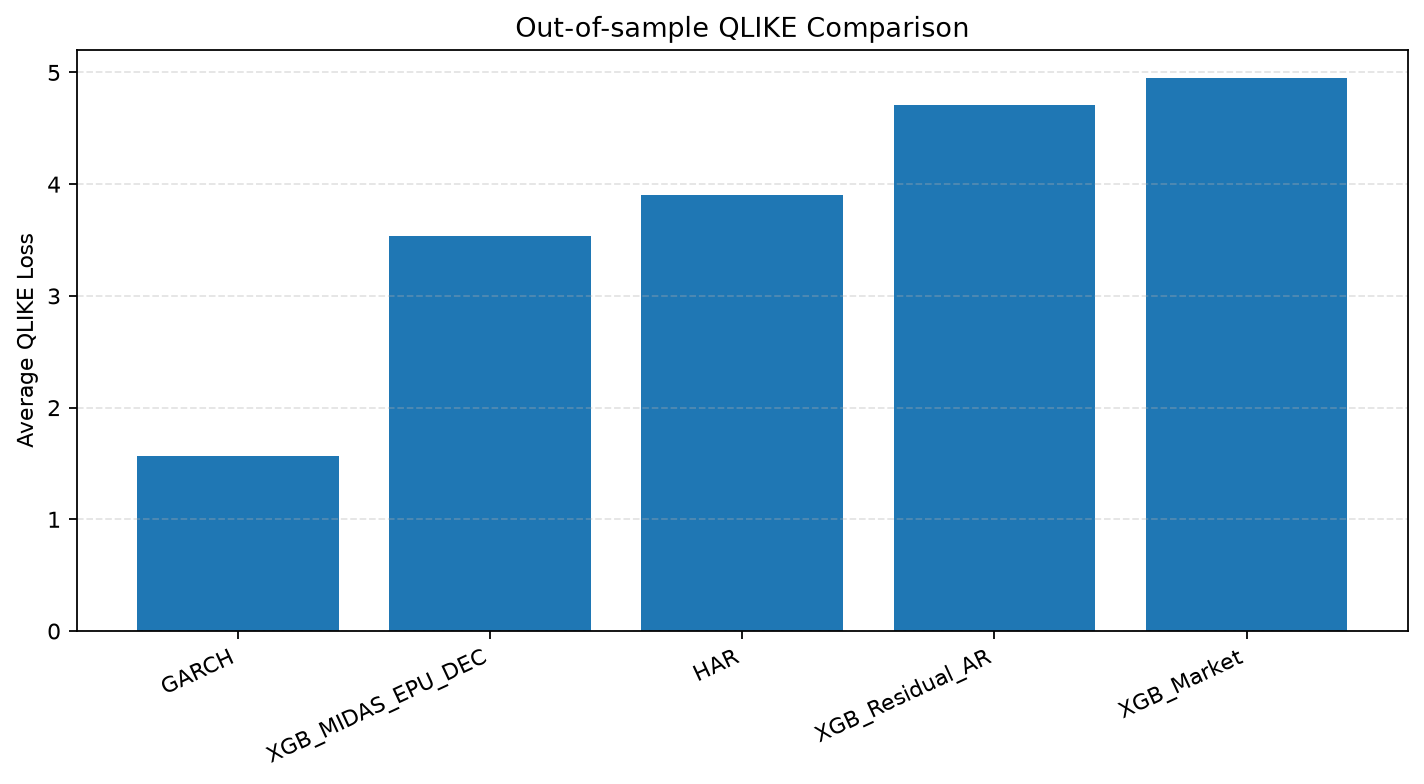
\includegraphics[width=.88\textwidth]{../../results/revised/csi300/fig_metrics_bar.png}
\caption{CSI300修订结果：五模型的QLIKE}\label{fig:metrics_bar}\end{figure}

\subsection{预测路径与累计损失}
近期路径及累计QLIKE差见图\ref{fig:prediction_series}和图\ref{fig:cumulative_qlike}。累计差定义为基准损失减DEC损失，曲线上升表示累计差向DEC有利方向变化；累计曲线不证明每一天均改善，也不能排除极端日期的影响。路径较平滑不能单独证明模型有效。
\begin{figure}[htbp]\centering
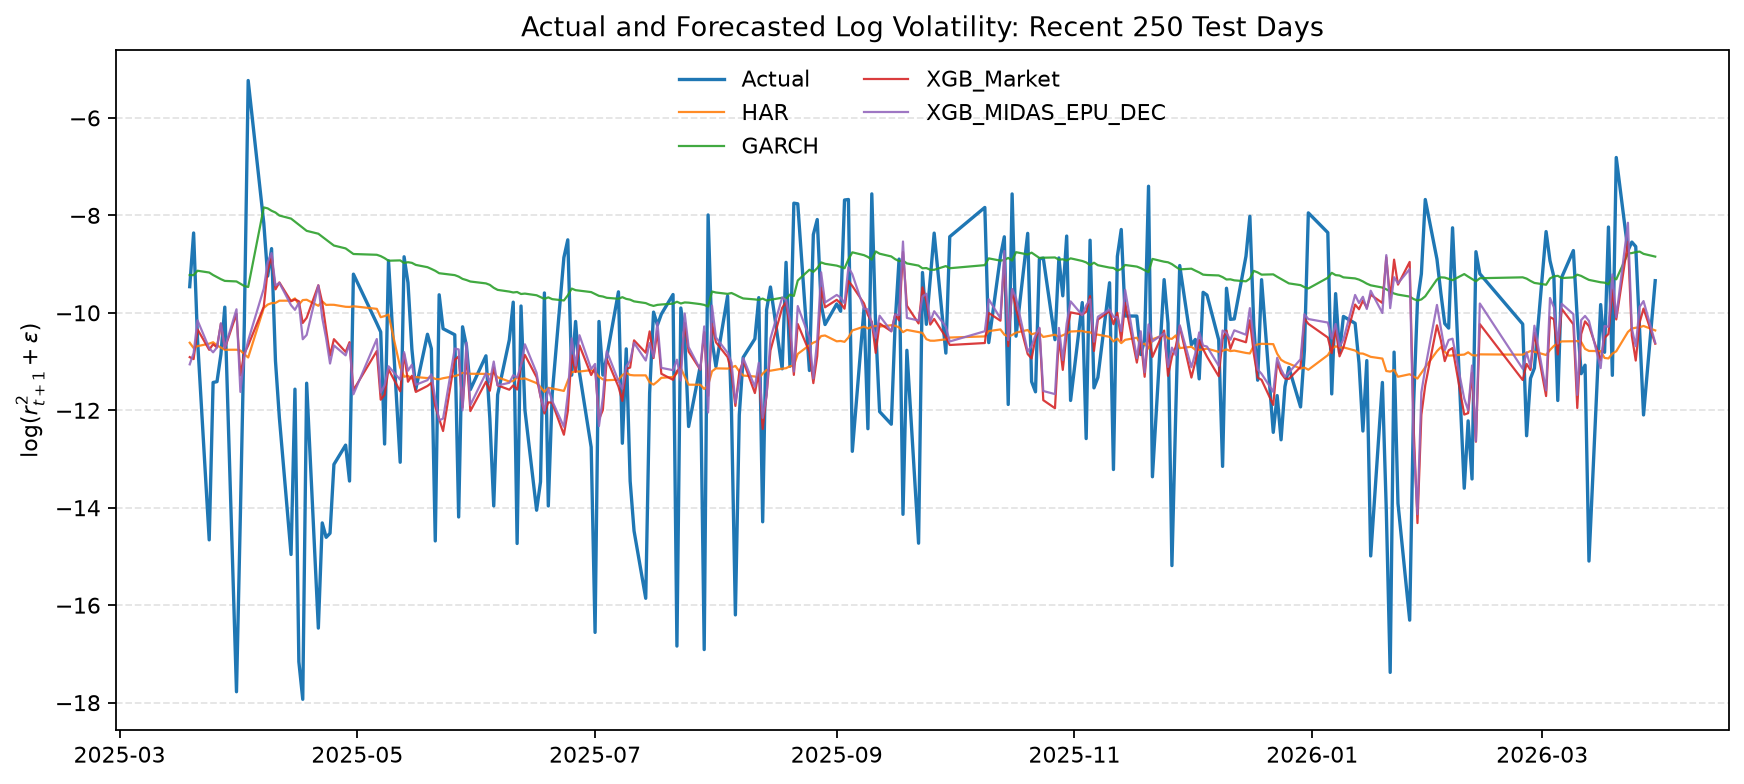
\includegraphics[width=.88\textwidth]{../../results/revised/csi300/fig_prediction_series_recent.png}
\caption{修订DEC与三个基准的近期预测路径}\label{fig:prediction_series}\end{figure}
\begin{figure}[htbp]\centering
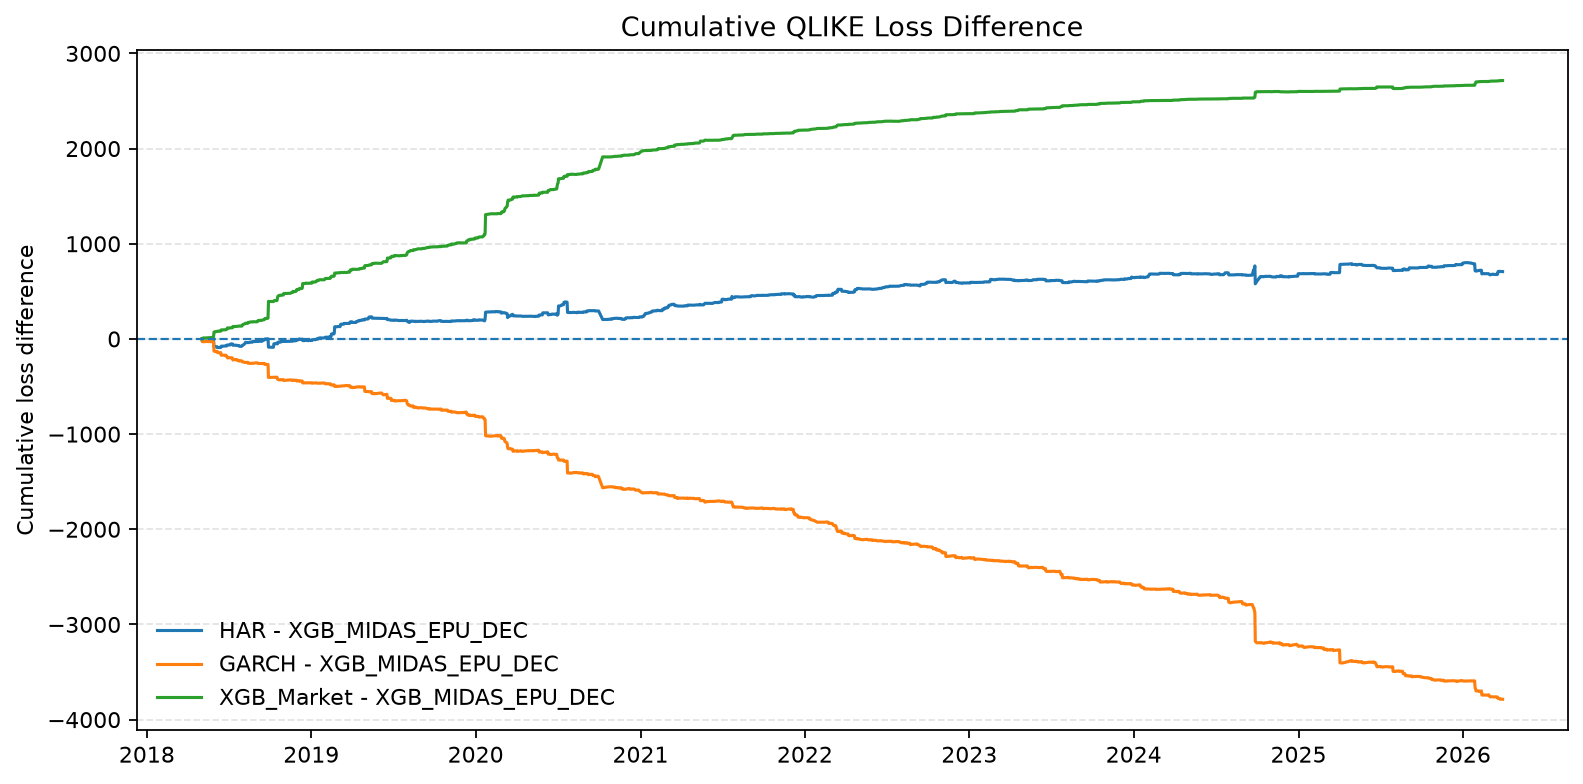
\includegraphics[width=.88\textwidth]{../../results/revised/csi300/fig_cumulative_qlike_diff.png}
\caption{修订DEC相对三基准的累计QLIKE差}\label{fig:cumulative_qlike}\end{figure}

\subsection{损失差诊断与统计解释}
表\ref{tab:hypothesis_tests}给出CSI300六项比较。正的平均损失差表示DEC更低；Holm调整覆盖三个市场的全部18项。MAE和QLIKE的差异在这些探索性参考值下较明确，MSE差异没有相应证据。模型选择及近似嵌套限制仍然存在，不能把调整后的$p$值当作完全有效的确认性检验。
\begin{table}[htbp]\centering\caption{CSI300损失差的探索性HAC诊断}\label{tab:hypothesis_tests}
\begin{tabular}{llrrr}\toprule 比较对象 & 损失 & 均值差 & HAC标准误 & Holm $p$\\\midrule
XGB-Market & MSE & -0.012928 & 0.041430 & 1\\
XGB-Market & MAE & 0.037528 & 0.008207 & 6.73e-05\\
XGB-Market & QLIKE & 1.414672 & 0.197725 & 1.43e-11\\
XGB-AR & MSE & -0.018475 & 0.035984 & 1\\
XGB-AR & MAE & 0.032464 & 0.007137 & 7.01e-05\\
XGB-AR & QLIKE & 1.168972 & 0.160859 & 6.61e-12\\
\bottomrule\end{tabular}\end{table}

\subsection{规格选择、权重及数值敏感性}
CSI300仍选24个月指数Almon。规格选择段的参数见表\ref{tab:midas_spec}，实际测试期每60条重新估计，因此图\ref{fig:midas_weights}不是固定全样本经济效应。参数触及边界也提示权重形状依赖约束，不能据其解释政策传导期限。
\begin{table}[htbp]\centering\caption{CSI300修订验证集所选规格}\label{tab:midas_spec}
\begin{tabular}{lrrrr}\toprule 权重族 & K & $\theta_1$ & $\theta_2$ & 验证MSE\\\midrule
指数Almon & 24 & 5.000000 & -4.488853 & 5.722685\\\bottomrule\end{tabular}\end{table}
\begin{figure}[htbp]\centering
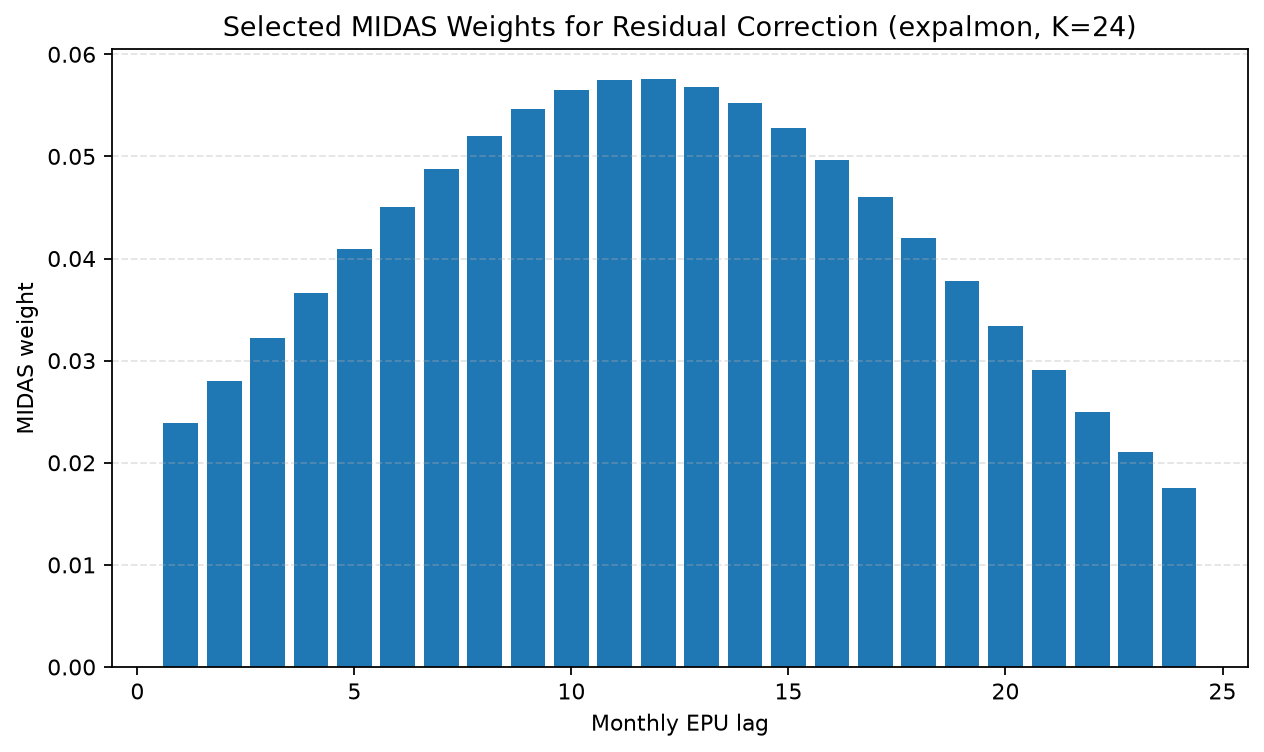
\includegraphics[width=.88\textwidth]{../../results/revised/csi300/fig_midas_weights.png}
\caption{修订后的CSI300验证选择权重}\label{fig:midas_weights}\end{figure}

旧存档DEC的MSE为5.112383、QLIKE为3.538317；修订后分别为5.112644和3.536964。MSE略差、QLIKE略好，不构成全面提升。修订理由是明确的数值估计缺陷和可复核的优化诊断，而不是追求较好看的测试成绩。附录和项目记录分别列出旧环境复现差异、固定规格控制以及新方法的跨依赖检查。

\subsection{本章小结}
CSI300支持保留传统基准，同时表明DEC的样本优势依赖评价损失。新增消融使“含EPU的组合与仅含残差的组合有何不同”可以直接比较；结论仍限定于当前数据、回顾性设计和预先固定的本轮求解规则。对区间质量是否有改善，需要单独检验。

\section{波动率区间预测结果分析与检验}

在前一章中，主要从点预测角度比较了 HAR、GARCH(1,1)、XGB-Market、XGB-AR以及XGB-MIDAS-EPU-DEC五类模型的样本外预测表现。点预测能够反映模型对未来波动率条件水平的刻画能力，但在金融风险管理、资产配置和极端风险预警场景中，仅报告点预测值是不充分的。原因在于，投资者和风险管理者不仅关心未来波动率的条件均值或条件中位水平，也关心预测误差可能处于何种范围之内。因此，在点预测结果之外，进一步构造预测区间能够更完整地评价模型对未来不确定性的刻画能力。

预测区间评价需要同时考虑两个维度：一是区间能否覆盖真实观测值，即有效性；二是在满足合理覆盖率的前提下，区间是否足够窄，即有效性约束下的精确性。若区间过宽，即使覆盖率较高，其实际风险管理价值也有限；若区间过窄，则可能频繁低估真实波动风险。因此，本文在五类点预测模型的基础上，进一步采用滚动共形预测方法构造波动率预测区间，并从经验覆盖率、平均区间宽度、区间得分以及滚动覆盖率等角度对模型进行比较。

本章检验修订DEC是否改善XGB-Market与XGB-AR的区间质量，不预设点预测中的部分指标优势会传递到预测区间。

\subsection{滚动共形预测方法}

本文采用基于历史预测残差的滚动共形预测方法构造区间。共形预测的基本思想是利用校准样本中的预测误差分布，对未来点预测值进行非参数修正，从而得到具有经验覆盖含义的预测区间。经典共形预测方法具有分布无关的优点，在独立同分布或可交换性假设下可以提供有限样本覆盖保证 \citep{Vovk2005,ShaferVovk2008,Lei2018}。然而，金融时间序列通常存在自相关、波动聚集和分布漂移，严格的可交换性假设难以满足。因此，本文不对金融时间序列下的共形区间作过强的有限样本精确覆盖声明，而是将其作为一种按保存预测的日期顺序进行校准的经验区间构造方法；这不验证上游点预测输入的实时可得性。

具体而言，设某一模型在时点 \(t-1\) 对 \(y_t\) 的点预测为 \(\hat{y}_{t|t-1}\)，则预测残差为
\begin{equation}
	e_t = y_t - \hat{y}_{t|t-1}.
\end{equation}
本文采用绝对误差作为非符合度分数：
\begin{equation}
	s_t = |e_t|.
\end{equation}

对于测试集中的任一预测时点 \(t\)，本文仅使用验证集残差和已经实现的历史测试集残差作为校准样本，并取最近 \(m\) 个非符合度分数计算经验分位数。设滚动校准窗口为 \(\mathcal{C}_t\)，其样本量为 \(n_t\)，则 \(1-\alpha\) 预测区间所需的共形分位数为
\begin{equation}
	q_{1-\alpha,t}
	=
	s_{\left(\lceil (n_t+1)(1-\alpha)\rceil\right)},
\end{equation}
其中 \(s_{(k)}\) 表示将校准窗口内非符合度分数从小到大排列后的第 \(k\) 个顺序统计量。若 \(\lceil (n_t+1)(1-\alpha)\rceil>n_t\)，代码将阶数截断至样本量并取最大分数；此做法不提供一般覆盖保证，本实验的窗口与显著性水平不触发这一边界。

在对数波动率尺度上，模型的一步超前预测区间定义为
\begin{equation}
	\left[
	L^{(y)}_{t+1|t},
	U^{(y)}_{t+1|t}
	\right]
	=
	\left[
	\hat{y}_{t+1|t}-q_{1-\alpha,t},
	\hat{y}_{t+1|t}+q_{1-\alpha,t}
	\right].
\end{equation}

本文采用滚动校准而非固定校准，主要基于两点考虑。第一，金融市场波动率的误差分布具有明显时变性，固定校准窗口可能无法及时反映近期市场状态。第二，滚动校准仅使用预测时点之前的近期误差信息，能够在经验上缓解时间序列非平稳性对共形覆盖的影响。类似地，已有时间序列共形预测研究也强调需要对动态序列中的依赖性和分布变化进行适应性处理 \citep{XuXie2021}。

\subsection{区间预测评价指标}

本文从经验覆盖率、平均区间宽度和区间得分三个角度评价预测区间质量。

首先，经验覆盖率定义为
\begin{equation}
	CP_{1-\alpha}
	=
	\frac{1}{N}
	\sum_{t=1}^{N}
	\mathbf{1}
	\left\{
	L^{(y)}_{t+1|t}
	\leq
	y_{t+1}
	\leq
	U^{(y)}_{t+1|t}
	\right\},
\end{equation}
其中 \(N\) 表示测试集评价样本量。经验覆盖率接近名义覆盖率 \(1-\alpha\) 是样本校准表现；需结合抽样误差、违约依赖与其他设置检验，不能单独据此证明区间有效。

其次，平均区间宽度定义为
\begin{equation}
	AW_{1-\alpha}
	=
	\frac{1}{N}
	\sum_{t=1}^{N}
	\left(
	U^{(y)}_{t+1|t}
	-
	L^{(y)}_{t+1|t}
	\right).
\end{equation}
在覆盖率相近的情况下，平均区间宽度越小，说明区间越精确。

最后，本文采用区间得分综合评价区间质量。该指标同时惩罚区间过宽和覆盖失败，是预测区间评价中常用的严格适当评分规则之一 \citep{GneitingRaftery2007}。对于显著性水平 \(\alpha\)，单期区间得分定义为
\begin{equation}
	\begin{aligned}
		IS_{\alpha,t+1}
		=
		&
		\left(
		U^{(y)}_{t+1|t}
		-
		L^{(y)}_{t+1|t}
		\right)
		\\
		&
		+
		\frac{2}{\alpha}
		\left(
		L^{(y)}_{t+1|t}
		-
		y_{t+1}
		\right)
		\mathbf{1}
		\left\{
		y_{t+1}<L^{(y)}_{t+1|t}
		\right\}
		\\
		&
		+
		\frac{2}{\alpha}
		\left(
		y_{t+1}
		-
		U^{(y)}_{t+1|t}
		\right)
		\mathbf{1}
		\left\{
		y_{t+1}>U^{(y)}_{t+1|t}
		\right\}.
	\end{aligned}
\end{equation}
样本平均区间得分为
\begin{equation}
	\overline{IS}_{\alpha}
	=
	\frac{1}{N}
	\sum_{t=1}^{N}
	IS_{\alpha,t+1}.
\end{equation}
该指标数值越低，说明区间预测质量越高。

此外，本文还采用 Christoffersen 的区间预测检验框架，对区间违约序列进行无条件覆盖、独立性和条件覆盖检验 \citep{Christoffersen1998}。其中，无条件覆盖检验关注违约比例是否与名义水平一致；独立性检验关注违约是否存在聚集；条件覆盖检验则同时考察覆盖率正确性和违约独立性。该检验尤其适合金融风险预测场景，因为在金融市场中，区间失效若集中发生在高波动时期，其实际风险含义通常比随机分散的少量失效更严重。

\subsection{共同日期上的主设置结果}
五模型均重新构造区间。DEC和XGB-AR没有验证段修正预测，须先积累60条测试残差；每组设置都取五模型共同的1859个日期，2018年7月27日至2026年3月30日。其余模型仍可使用自己的历史验证残差校准，只统一评价日期，不丢弃可用历史信息。所有表、图和覆盖检验采用这一相同日期口径。

\begin{table}[htbp]\centering\caption{共同日期的90\%区间，窗口250}\label{tab:interval_main}\label{tab:common_intervals}
\begin{tabular}{lrrrr}\toprule
模型 & N & 覆盖率 & 宽度 & 得分 \\
\midrule
HAR & 1859 & 0.9005 & 6.9949 & 9.6973 \\
GARCH(1,1) & 1859 & 0.8967 & 9.1225 & 12.6634 \\
XGB-Market & 1859 & 0.8983 & 7.0644 & 9.8534 \\
XGB-AR & 1859 & 0.9021 & 7.0662 & 9.8793 \\
DEC & 1859 & 0.8989 & 7.0634 & 10.1995 \\
\bottomrule\end{tabular}\end{table}

DEC得分高于HAR、XGB-Market及XGB-AR，低于GARCH。DEC区间略窄于两个XGB对照，但区间得分更高；不能用微小宽度优势代替整体评分。该比较未进行区间得分差异的显著性检验。GARCH结果来自相同的对数残差区间算法，不是GARCH原生分布区间的评价。
\begin{figure}[htbp]\centering
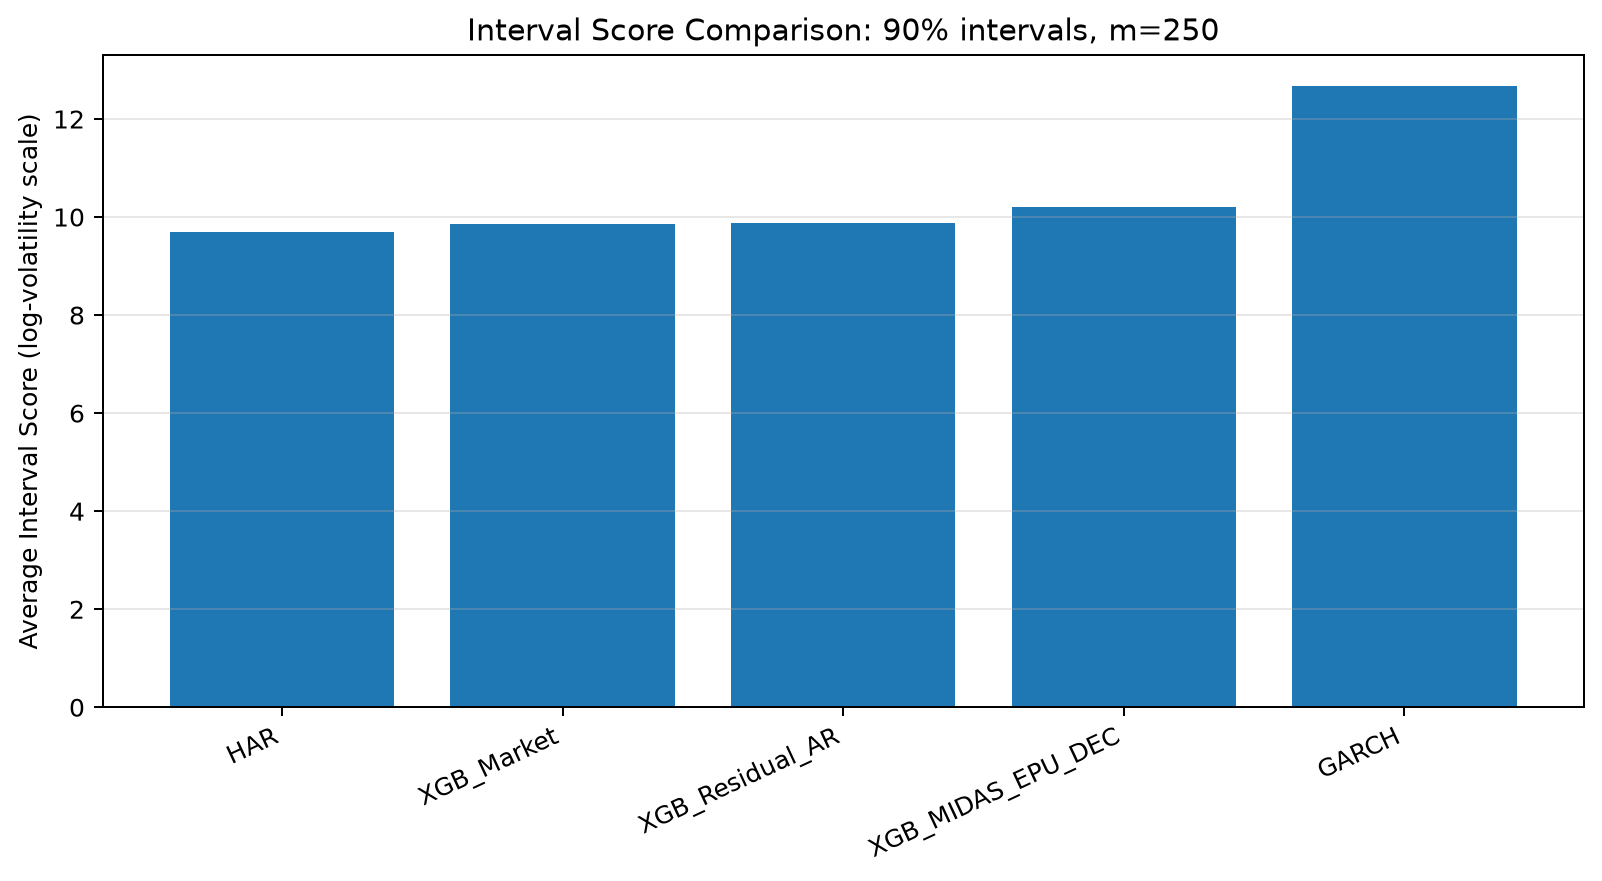
\includegraphics[width=.88\textwidth]{../../results/revised/intervals/fig_interval_score_main.png}
\caption{五模型共同日期上的区间得分}\label{fig:interval_score_main}\end{figure}
\begin{figure}[htbp]\centering
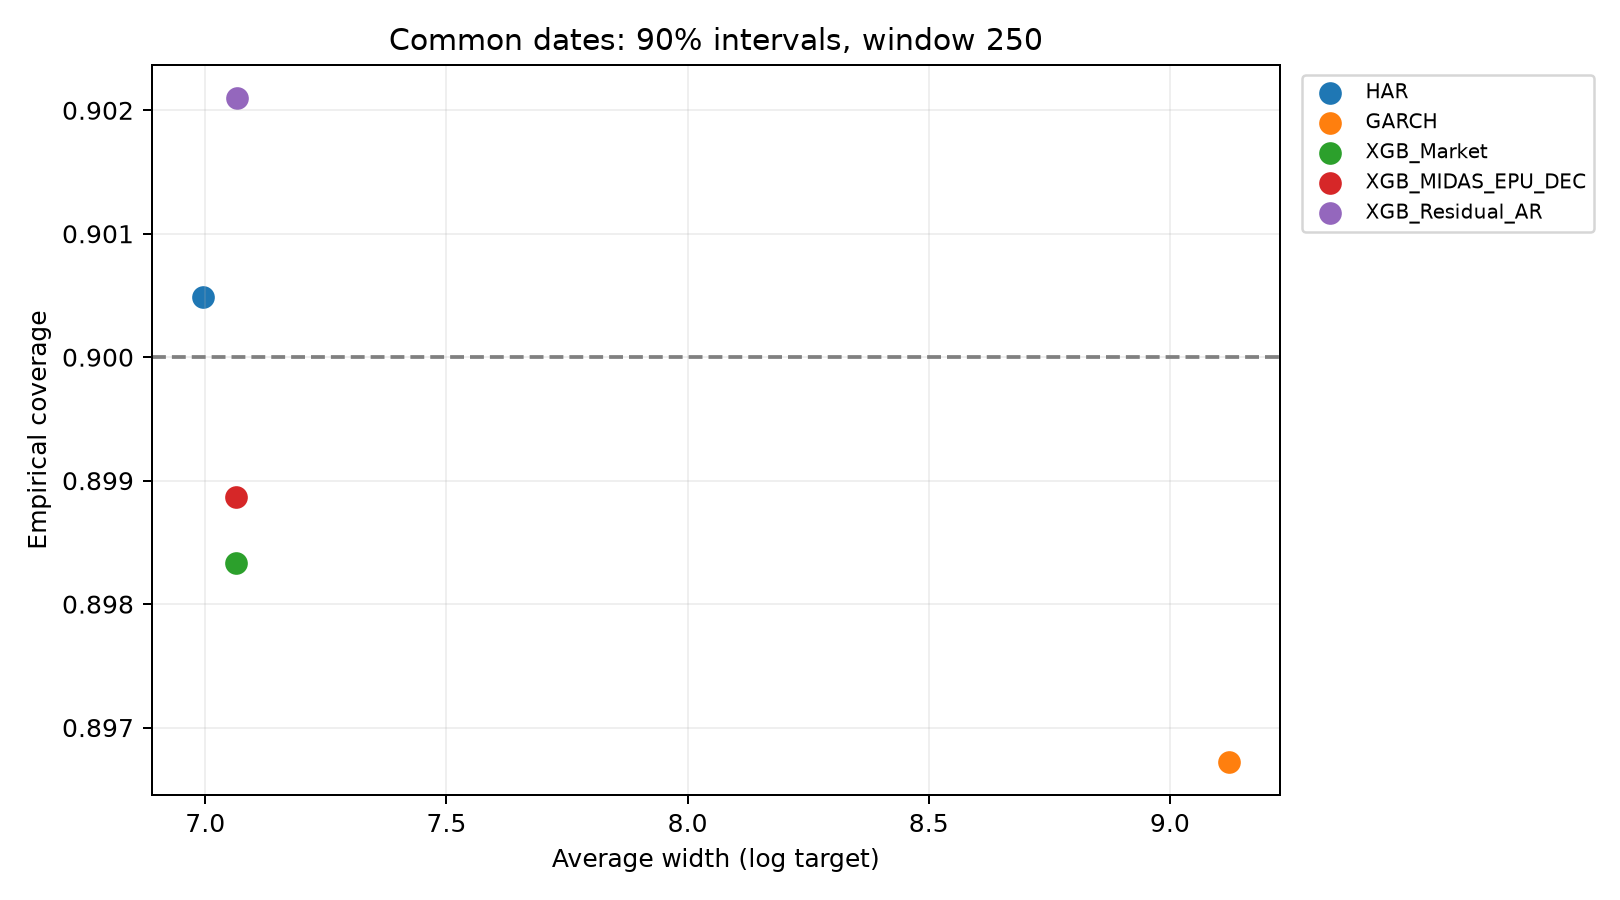
\includegraphics[width=.88\textwidth]{../../results/revised/intervals/fig_coverage_width_tradeoff_main.png}
\caption{共同日期上的覆盖率与区间宽度}\label{fig:coverage_width_tradeoff}\end{figure}

\subsection{覆盖检验及局部表现}
\begin{table}[htbp]\centering\caption{共同日期上的主设置覆盖诊断}\label{tab:christoffersen_main}
\begin{tabular}{lrrrr}\toprule
模型 & 违约数 & $p_{uc}$ & $p_{ind}$ & $p_{cc}$ \\
\midrule
HAR & 185 & 0.9445 & 0.1024 & 0.2629 \\
GARCH(1,1) & 192 & 0.6388 & 0.1370 & 0.2964 \\
XGB-Market & 189 & 0.8110 & 0.0987 & 0.2487 \\
XGB-AR & 182 & 0.7623 & 0.1896 & 0.4041 \\
DEC & 188 & 0.8712 & 0.0880 & 0.2303 \\
\bottomrule\end{tabular}\end{table}

主设置中五模型的UC、IND和CC参考检验均未在5\%水平拒绝。不拒绝不能证明正确覆盖，未对这些覆盖诊断进行多重检验调整。95\%区间、窗口120时，DEC的独立性$p=0.0062$、条件覆盖$p=0.0233$，仍提示违约聚集；不能只报告有利的主设置。

相邻60日覆盖窗口高度重叠。滚动覆盖率和近期区间路径仅展示样本动态，不能作为独立重复证据，也不能把全部未覆盖都归因于噪声或突然冲击。
\begin{figure}[htbp]\centering
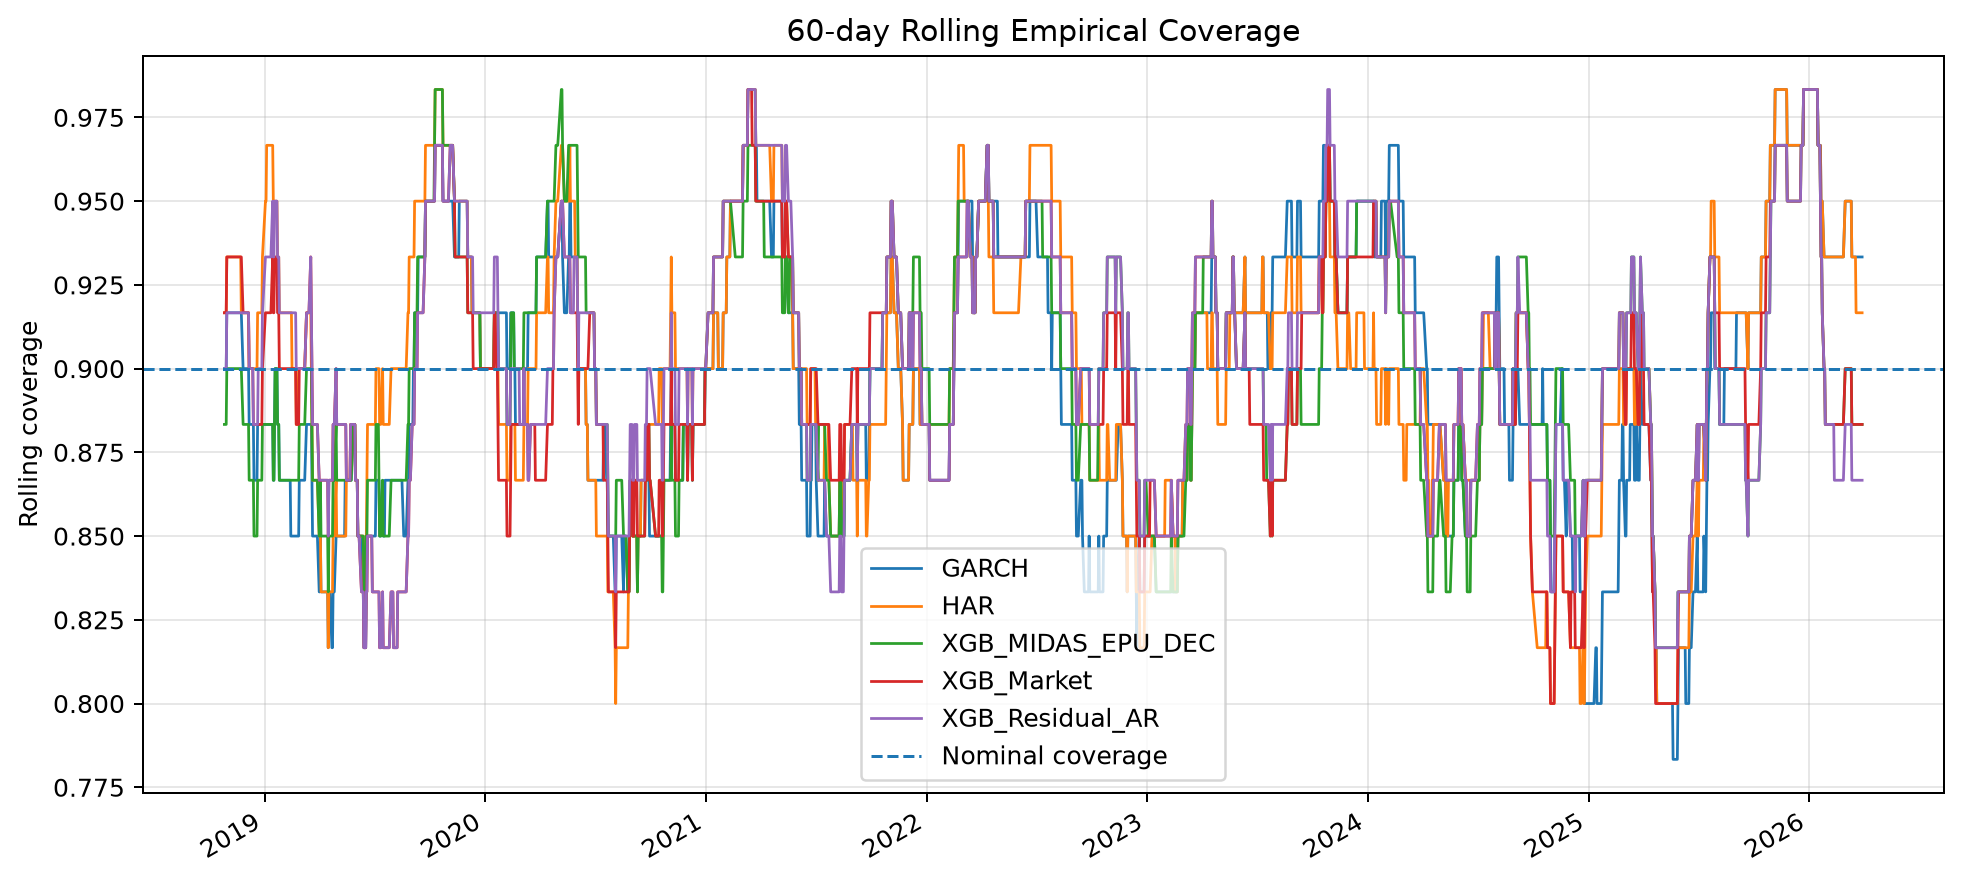
\includegraphics[width=.88\textwidth]{../../results/revised/intervals/fig_rolling_coverage_main.png}
\caption{共同评价段内60日滚动覆盖率}\label{fig:rolling_coverage}\end{figure}
\begin{figure}[htbp]\centering
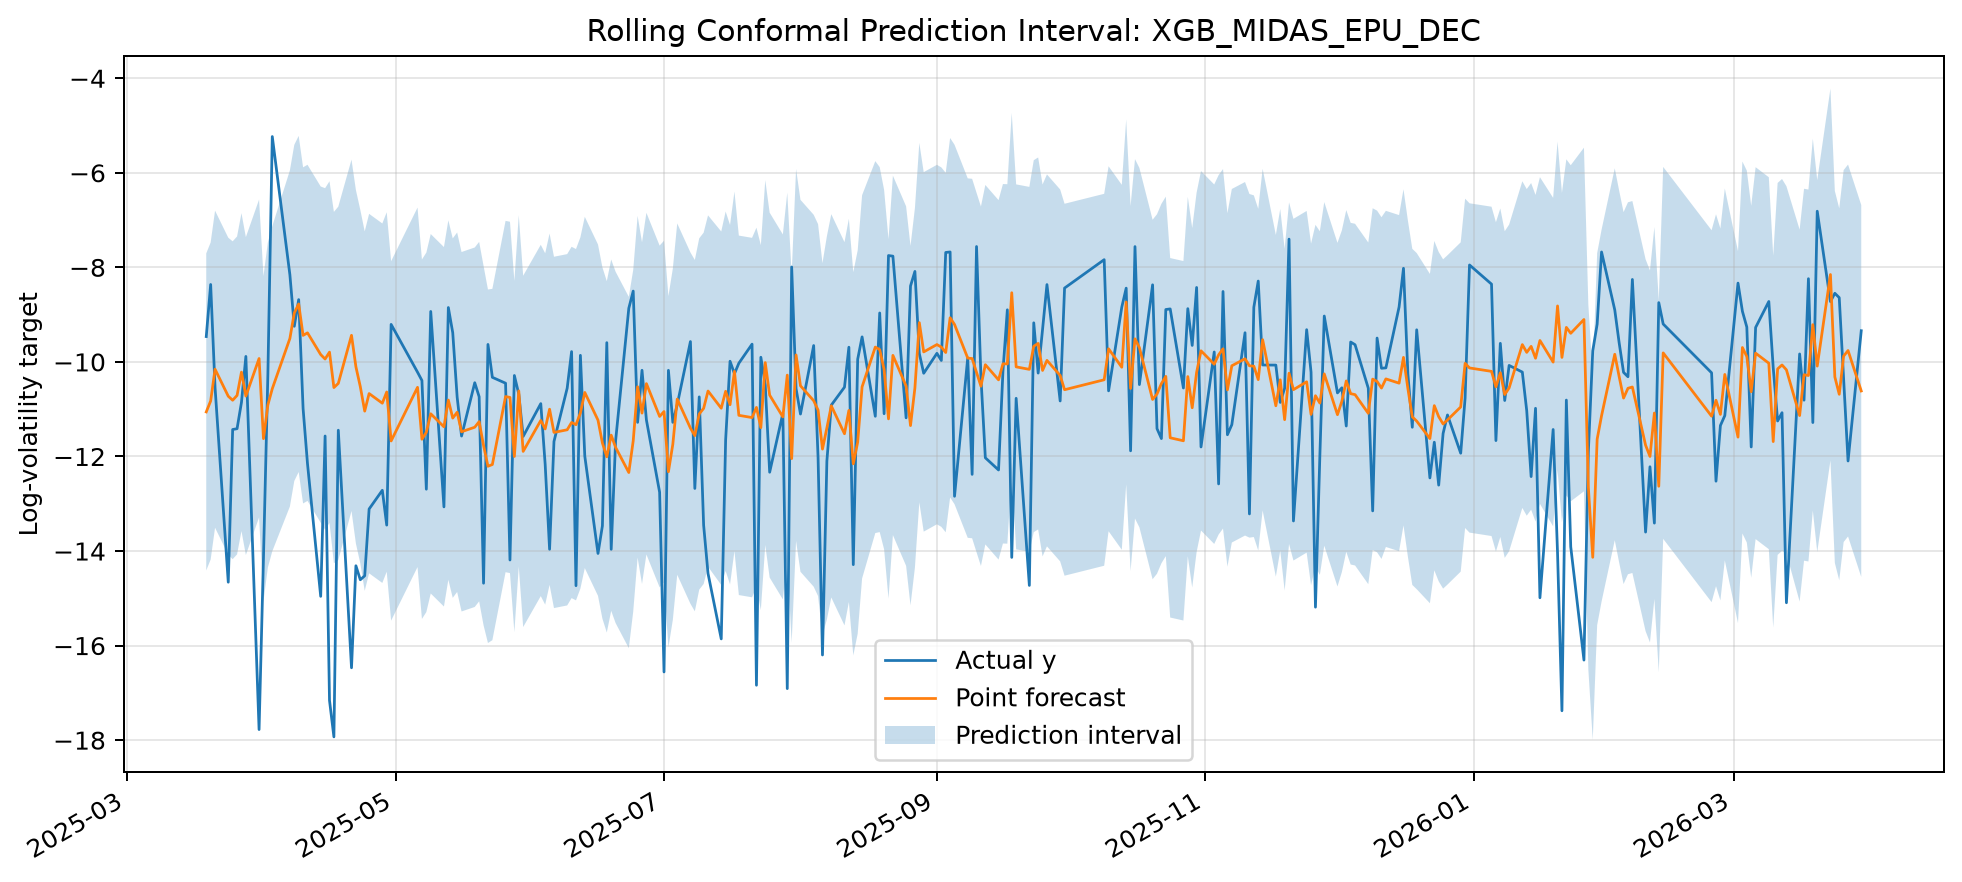
\includegraphics[width=.88\textwidth]{../../results/revised/intervals/fig_interval_series_XGB_MIDAS_EPU_DEC.png}
\caption{修订DEC的近期滚动残差区间}\label{fig:interval_series_xgb_midas}\end{figure}

\subsection{窗口与名义水平的敏感性}
\begin{table}[htbp]\centering\caption{共同日期上90\%区间的平均得分}\label{tab:interval_robustness}
\begin{tabular}{lrrr}\toprule 模型 & 窗口120 & 窗口250 & 窗口500\\\midrule
HAR & 9.7468 & 9.6973 & 9.6938\\
GARCH(1,1) & 12.6511 & 12.6634 & 12.6021\\
XGB-Market & 9.9336 & 9.8534 & 9.8528\\
XGB-AR & 9.9387 & 9.8793 & 9.8628\\
DEC & 10.2852 & 10.1995 & 10.1807\\
\bottomrule\end{tabular}\end{table}
六组名义水平与窗口设置、五模型共30组结果均随项目提供。排序和覆盖表现应按具体设置判断，不从单一主设置推广一般有效性。对CSI300而言，修订DEC的主设置得分由历史10.1991变为10.1995，略差；基准排序没有因数值修正而改变。

\subsection{本章小结}
修订DEC仍未改善XGB-Market及XGB-AR的区间质量。QLIKE改善与区间评分改善是不同命题；本文没有得到二者同时占优的证据。所有结论仅针对未来观测代理和本次滚动绝对残差构造，不能用于宣称潜在方差置信区间有效。

\section{替代市场的修订结果}
本章使用上证50与纳斯达克综合指数评价相同模型家族，并增加XGB-AR对照。上证50在特征构造前删除2018年6月18日已确认休市行，修订样本为1500/500/1919；纳斯达克保持2000/500/1554。上证50采用中国月度EPU，纳斯达克采用美国月度EPU，真实发布时间与历史修订版本均未完整保存。不同市场与训练长度限制横向解释，不能称为独立外部验证。

\subsection{修订的点预测结果}
\begin{table}[htbp]\centering\caption{上证50日历修正后的结果，N=1919}\label{tab:sse50_metrics}
\begin{tabular}{lrrr}\toprule
模型 & MSE & MAE & QLIKE \\
\midrule
HAR & 4.826226 & 1.717026 & 3.872429 \\
GARCH(1,1) & 7.537442 & 2.043060 & 1.586804 \\
XGB-Market & 4.940740 & 1.740321 & 4.753901 \\
XGB-AR & 4.954984 & 1.741490 & 4.697720 \\
DEC & 4.972472 & 1.718639 & 3.672557 \\
\bottomrule\end{tabular}\end{table}
\begin{table}[htbp]\centering\caption{纳斯达克修订结果，N=1554}\label{tab:nas_metrics}
\begin{tabular}{lrrr}\toprule
模型 & MSE & MAE & QLIKE \\
\midrule
HAR & 5.292393 & 1.814872 & 3.994306 \\
GARCH(1,1) & 7.110225 & 1.894212 & 1.498305 \\
XGB-Market & 5.284620 & 1.767569 & 4.279836 \\
XGB-AR & 5.302560 & 1.761263 & 4.224645 \\
DEC & 5.369943 & 1.772158 & 3.895152 \\
\bottomrule\end{tabular}\end{table}

上证50中DEC相对XGB-Market和XGB-AR降低QLIKE及MAE，但提高MSE。纳斯达克中DEC相对两个XGB对照降低QLIKE，却同时提高MSE及MAE。三个市场的QLIKE排序均为GARCH最低，DEC其次，再是HAR及两个XGB对照中的其余模型；具体次序见完整表。加入EPU的收益依赖损失函数，不能声称跨指标普遍优势。

\subsection{纳斯达克规格改变及其原因}
历史单起点Beta解在299条估计残差上的SSE约1780.2771，验证MSE约4.3325。多起点找到训练SSE约1779.2408的更低解，但其验证MSE升至5.0476；此时12个月指数Almon的验证MSE为4.3446，成为六候选中的最小值。因此本文按原有选择规则改用Almon，而不是根据测试QLIKE选择Beta。

若强行固定历史12个月Beta规格、只修正求解，纳斯达克测试MSE为5.434646、QLIKE为3.791512；按验证规则重选Almon则为5.369943和3.895152。旧局部解可能产生类似隐式正则化的有限样本效果，但这只是解释假说，不能成为宣称已正确最小化训练目标的依据。更可靠的数值求解不保证更好的测试预测。

相对历史DEC的5.423666和3.794736，修订Almon的MSE下降约0.99\%，QLIKE上升约2.65\%。变化应如实报告，不选择性只展示有利指标。上证50包含数据清洗和求解两种变化，不能把历史表与修订表的总差值全部归因于优化器；项目另提供同输入的数值控制。
\subsection{上证50的图形结果}
\begin{figure}[H]\centering
\begin{minipage}{0.48\textwidth}\centering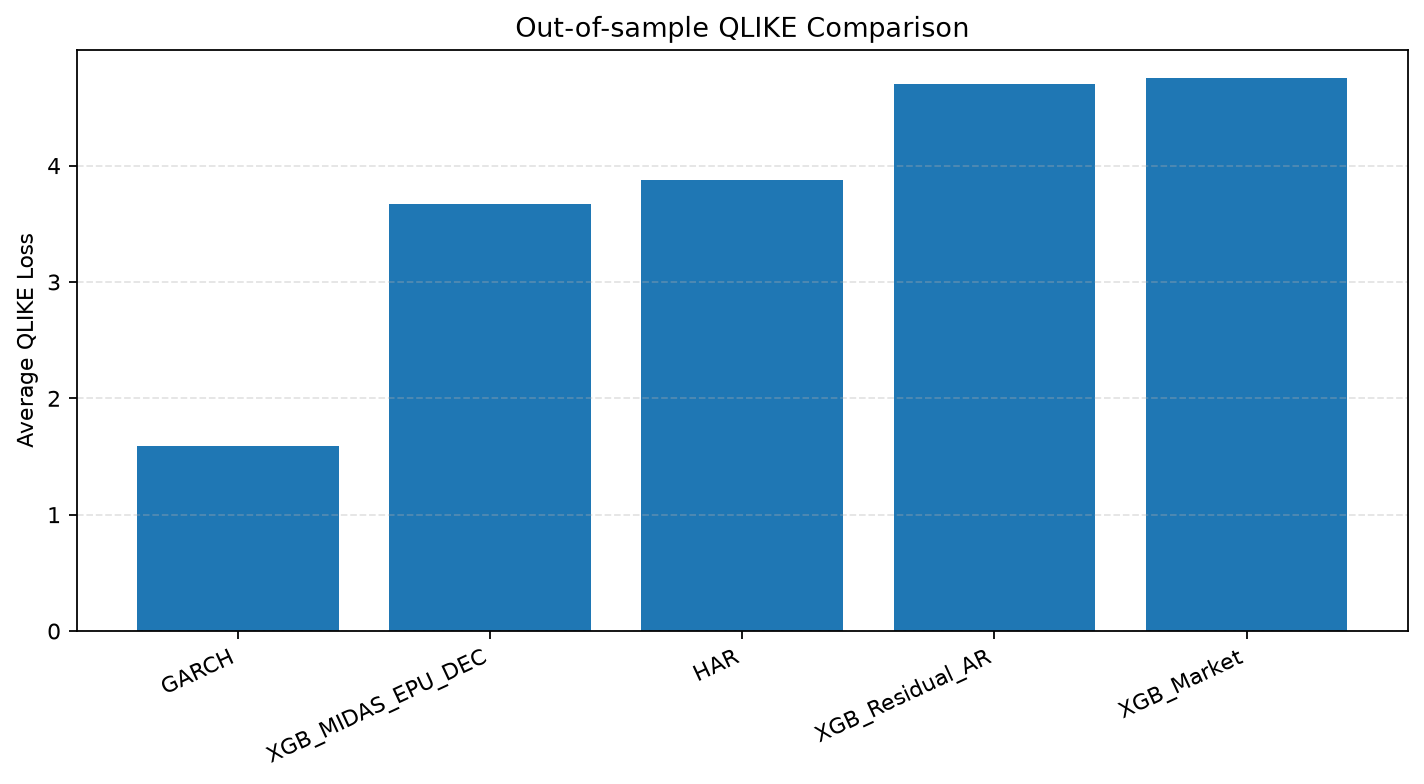
\includegraphics[width=\linewidth]{../../results/revised/sse50/fig_metrics_bar.png}\par{\small QLIKE}\end{minipage}\hfill
\begin{minipage}{0.48\textwidth}\centering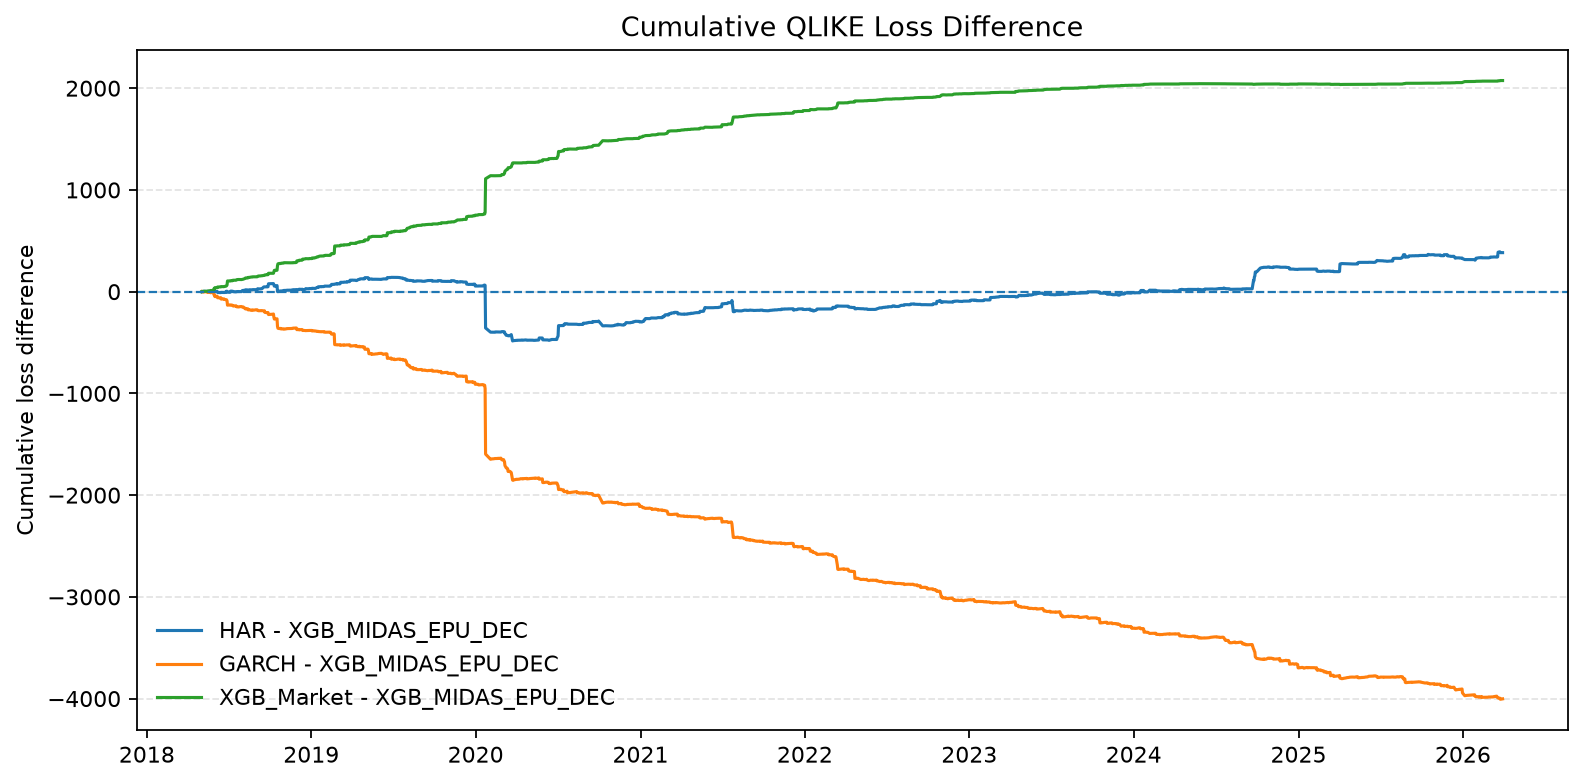
\includegraphics[width=\linewidth]{../../results/revised/sse50/fig_cumulative_qlike_diff.png}\par{\small 累计QLIKE差}\end{minipage}\par\medskip
\begin{minipage}{0.48\textwidth}\centering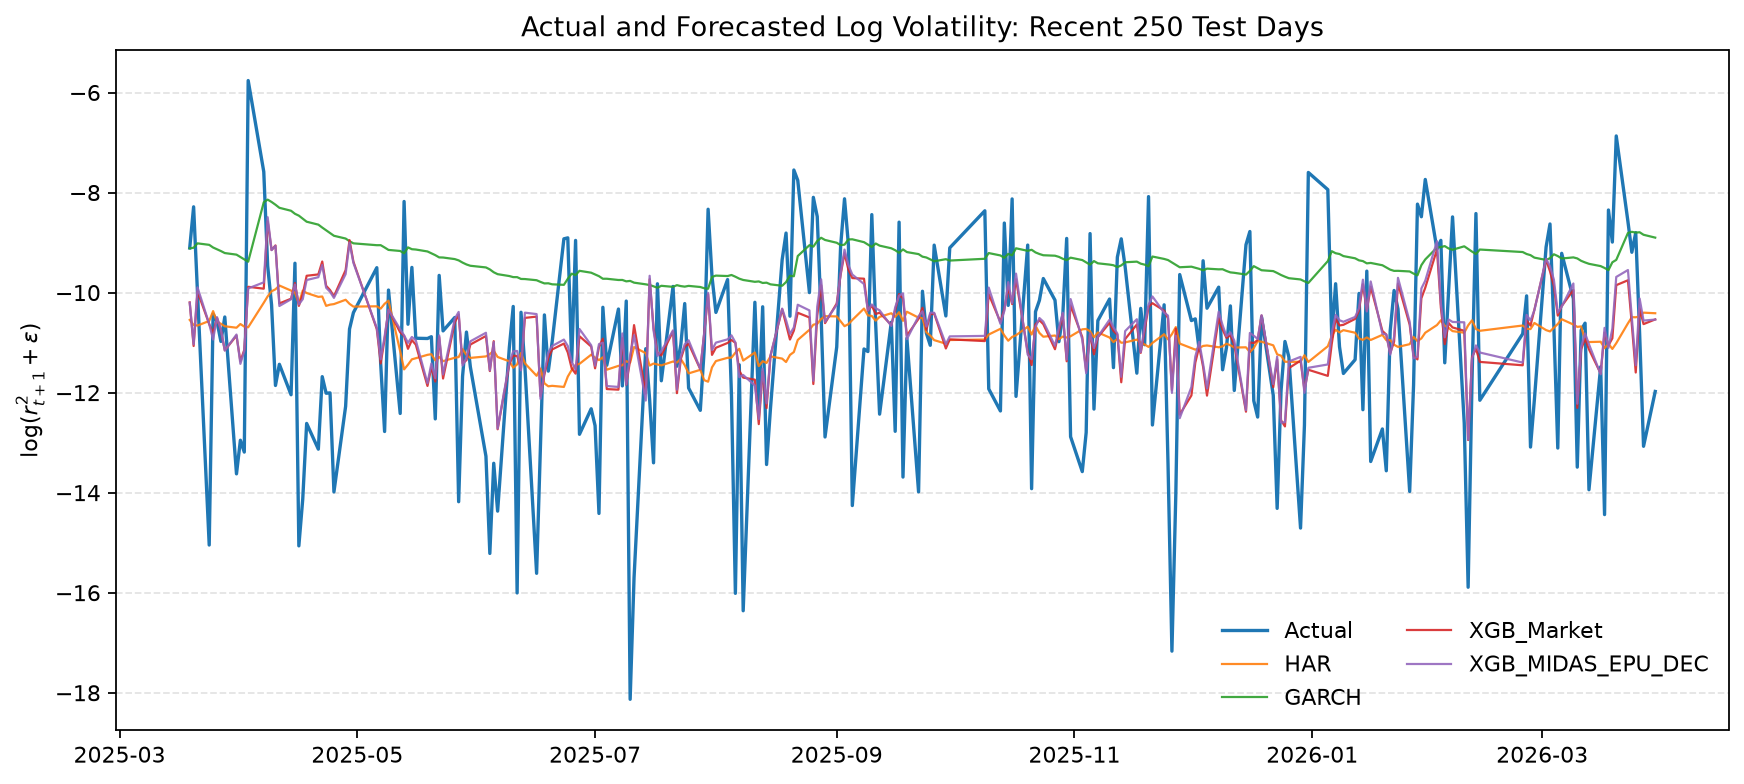
\includegraphics[width=\linewidth]{../../results/revised/sse50/fig_prediction_series_recent.png}\par{\small 近期预测}\end{minipage}\hfill
\begin{minipage}{0.48\textwidth}\centering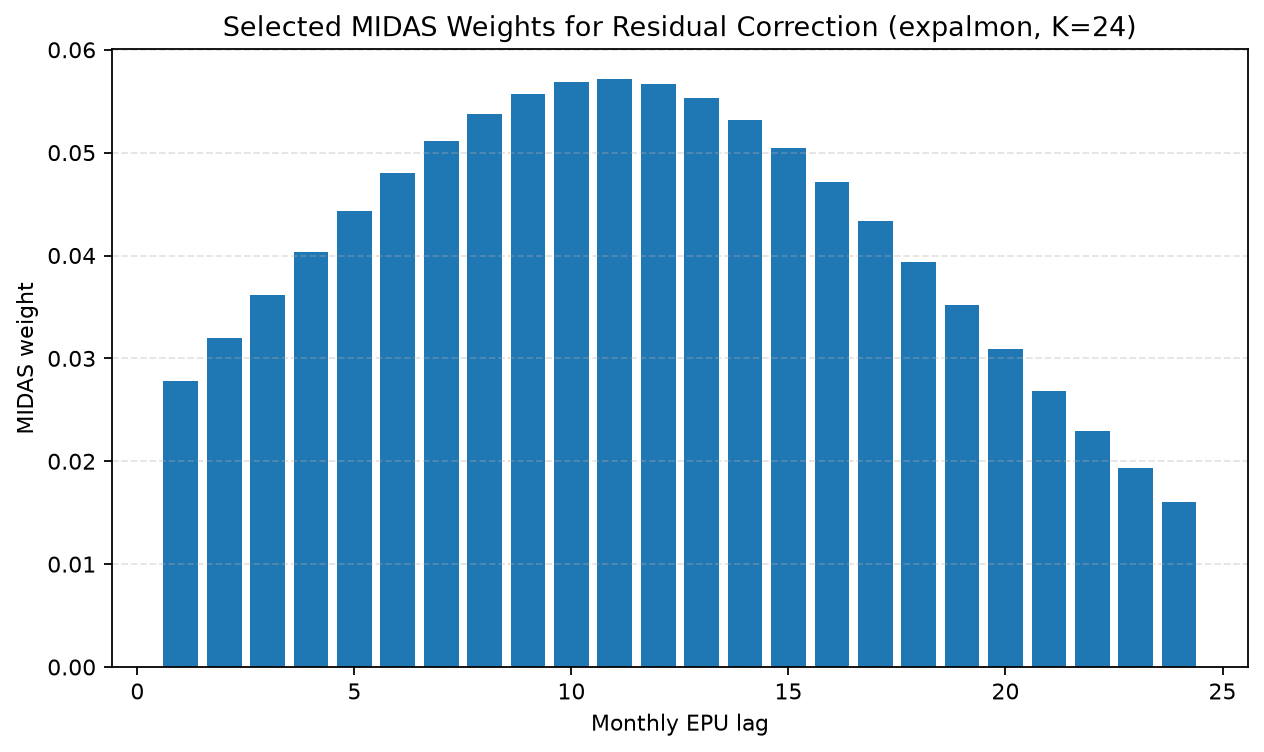
\includegraphics[width=\linewidth]{../../results/revised/sse50/fig_midas_weights.png}\par{\small 验证选择权重}\end{minipage}\par\medskip
\caption{上证50修订实验结果}\label{fig:sse50_robustness_panel}\end{figure}
\subsection{纳斯达克的图形结果}
\begin{figure}[H]\centering
\begin{minipage}{0.48\textwidth}\centering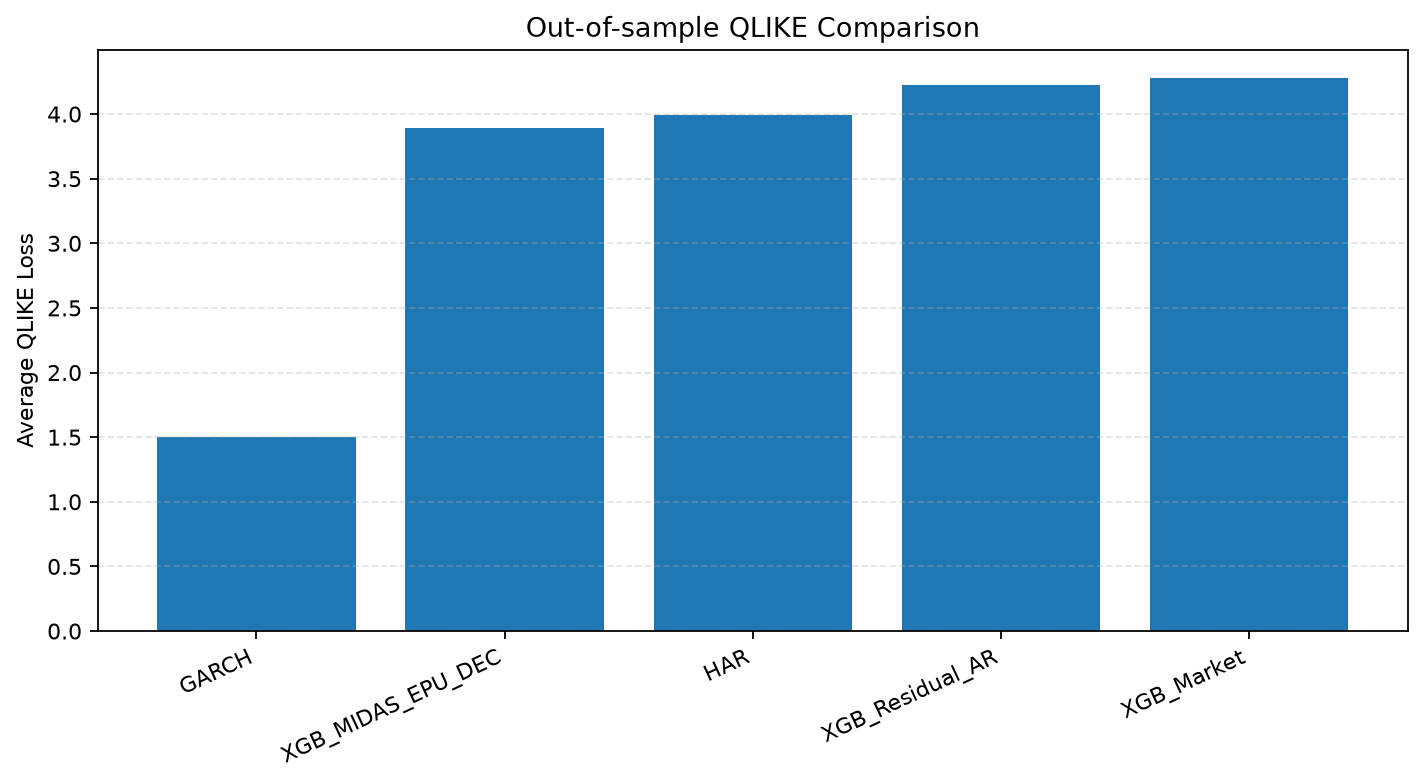
\includegraphics[width=\linewidth]{../../results/revised/nasdaq/fig_metrics_bar.png}\par{\small QLIKE}\end{minipage}\hfill
\begin{minipage}{0.48\textwidth}\centering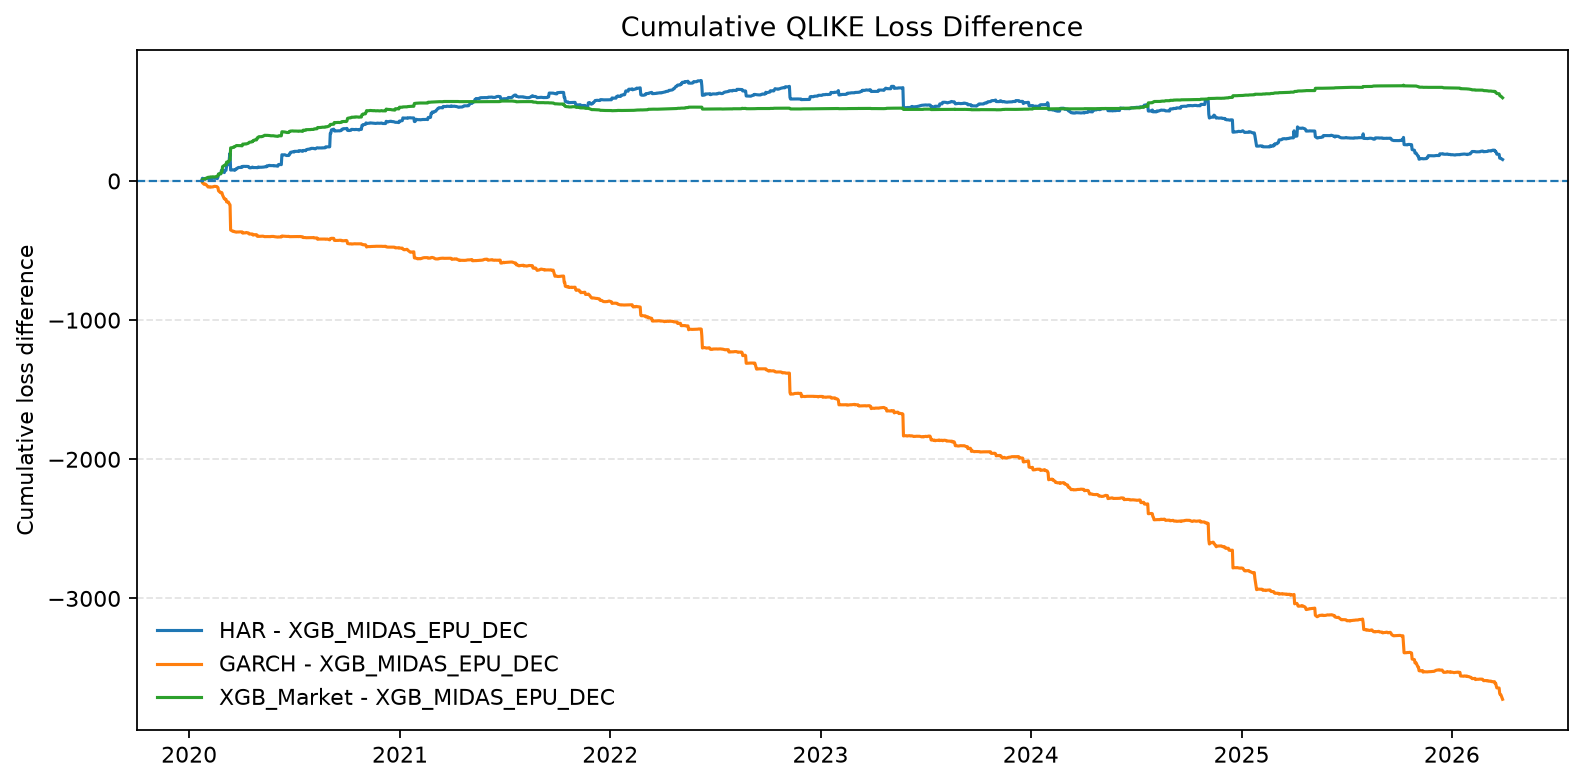
\includegraphics[width=\linewidth]{../../results/revised/nasdaq/fig_cumulative_qlike_diff.png}\par{\small 累计QLIKE差}\end{minipage}\par\medskip
\begin{minipage}{0.48\textwidth}\centering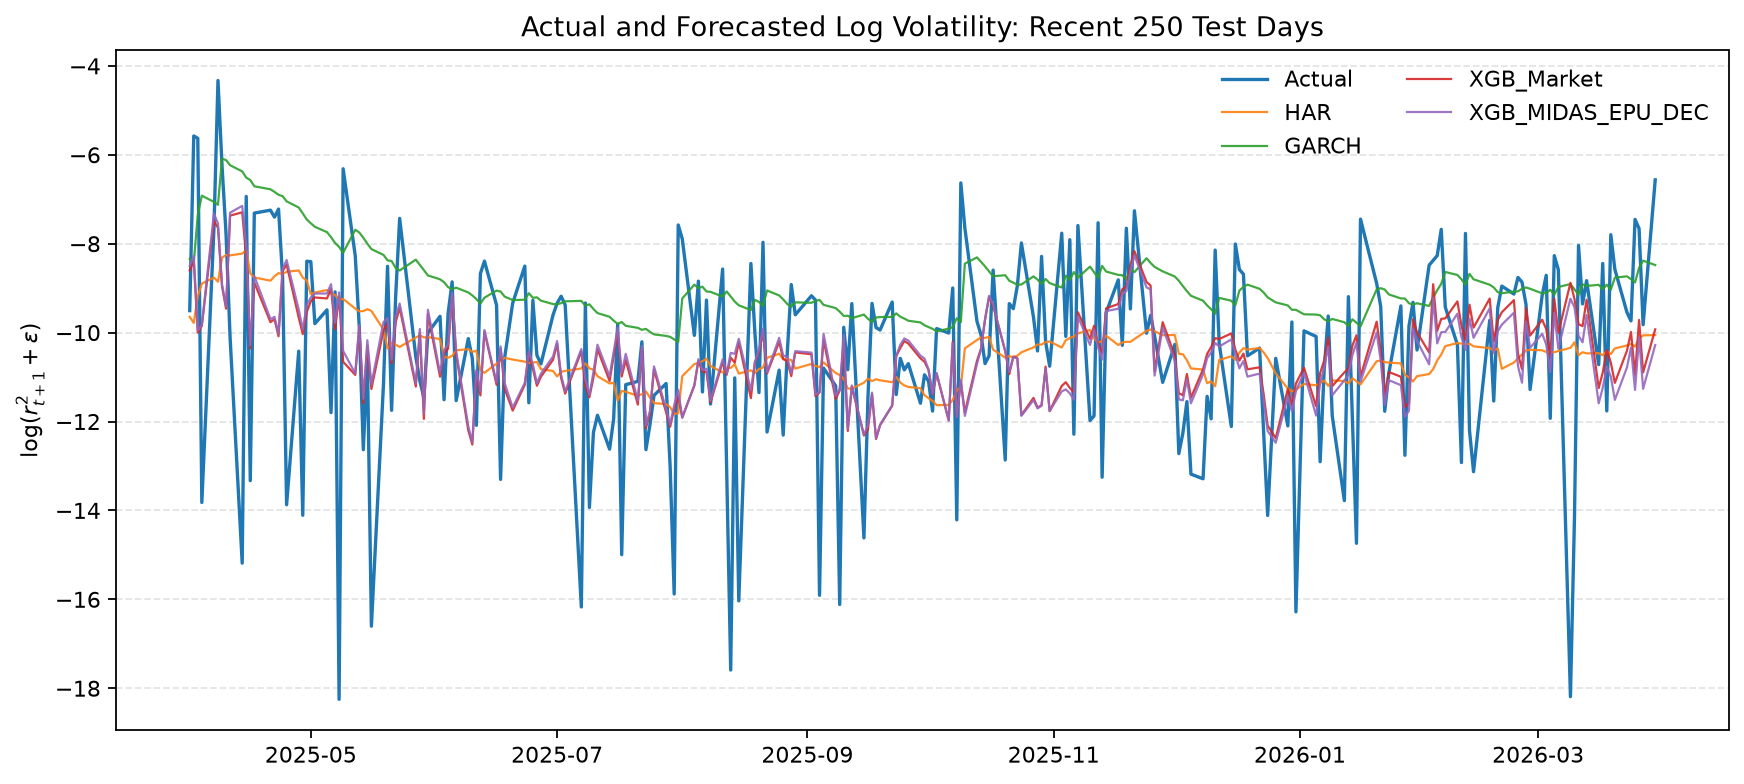
\includegraphics[width=\linewidth]{../../results/revised/nasdaq/fig_prediction_series_recent.png}\par{\small 近期预测}\end{minipage}\hfill
\begin{minipage}{0.48\textwidth}\centering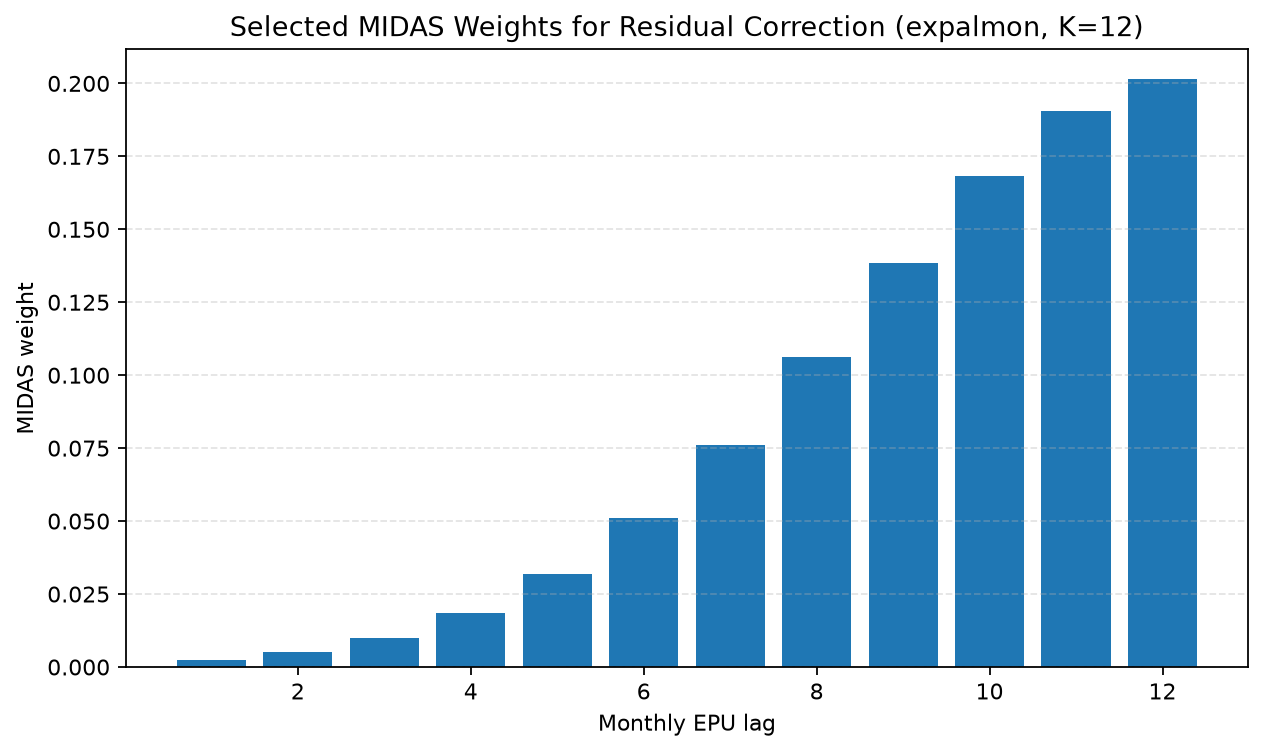
\includegraphics[width=\linewidth]{../../results/revised/nasdaq/fig_midas_weights.png}\par{\small 验证选择权重}\end{minipage}\par\medskip
\caption{纳斯达克修订实验结果}\label{fig:nas_robustness_panel}\end{figure}
\subsection{消融结果及解释范围}
三市场DEC相对XGB-AR的QLIKE均值差分别为1.168972、1.025163和0.329494；18项Holm调整后的正态参考$p$值分别约为$6.61\times10^{-12}$、$4.65\times10^{-7}$及0.0215。这是在回顾性、近似嵌套与规格选择限制下的探索性支持，不能升级为确定的总体优势。三市场MSE均较XGB-AR高，调整后没有支持MSE改善的证据。

中国两市场仍选择24个月指数Almon，纳斯达克改选12个月指数Almon。权重图展示验证阶段参数，测试期间会重估，边界解不应被解释为稳定政策传导机制。下一步应使用事先锁定的设计、独立时间留出集和真实发布版本的EPU，评估这些差异是否持续。

\clearpage\section*{结论}\addcontentsline{toc}{section}{结论}
本次公开修订将研究重点从复刻旧数值扩展到可靠估计和可解释比较。保留历史证据的同时，采用解析梯度与确定性多起点求解DEC，在上证50特征构造前排除已确认的休市行，并新增不含EPU的XGB-AR对照。沪深300中HAR的MSE、MAE最低，GARCH的QLIKE最低；DEC相对XGB-Market降低QLIKE和MAE，但MSE略高。

新增消融表明，三市场加入MIDAS-EPU后相对XGB-AR均降低QLIKE、提高MSE，中国两市场的MAE下降而纳斯达克上升。由此应将结论表述为当前设定下依赖损失函数的增量预测表现，不是EPU普遍改善预测或产生结构性因果效应。HAC和Holm调整提供探索性支持，不能消除回顾性分析、非线性估计及规格选择的推断限制。

纳斯达克验证最优规格从旧版12个月Beta改为12个月指数Almon。旧Beta局部解的训练目标更高，却偶然具有更低的验证误差；修订求解后按相同验证规则重选规格。相对旧DEC，修订测试MSE下降而QLIKE上升。这说明方法修正的价值在于估计规则清楚、数值更稳定和证据可追溯，并不要求所有测试指标都改善。

共同1859个日期上，主设置的DEC区间得分为10.1995，高于HAR的9.6973、XGB-Market的9.8534和XGB-AR的9.8793。DEC没有改善这些基准的区间质量。主设置覆盖诊断不拒绝不构成有效性证明；95\%、窗口120的DEC仍有违约独立性及条件覆盖拒绝结果。区间只针对观测代理及统一残差构造。

数值追溯已经精确重现6888条历史XGBoost预测；旧DEC历史环境仍不能唯一还原，新DEC在两套数值依赖中的最大预测差异小于$10^{-7}$。多起点不保证全局最优，边界权重的经济解释应克制。描述统计已使用3941条真实有效收益率；其他日期质量、EPU实时发布与修订、对数反变换以及独立样本表现仍待核验。未来应以这些问题及确认性留出评估为重点，不将当前结果包装成已验证的实时预测系统。

\clearpage\phantomsection\addcontentsline{toc}{section}{参考文献}
\nocite{*}\bibliographystyle{plainnat}\bibliography{../references}
\clearpage\appendix
\section{训练配置、平台抽样与复现证据}
现存主脚本与历史讨论记录均使用深度4、300棵树的设定。先前仅切换Python依赖版本仍未匹配；进一步保持参数与输入不变，只替换列抽样中的平台洗牌实现后，XGBoost 2.0.3的CPU直方图训练逐点重现三个市场共6888条存档预测。兼容实现采用Microsoft STL 17.6的列洗牌规则，保留原mt19937随机引擎；没有调整随机种子来追拟合历史结果，也没有把测试损失用于选参。原生macOS抽样作为对照仍不匹配。

这确认了一套能生成全部存档XGBoost预测的数值等价配置，支持现存主脚本与最终结果对应；它不能唯一确定当时安装的版本、编译器或全部系统库。原稿附录中的深度3、最小子节点权重5、L1系数0及早停50不适合作为最终实验说明，现以匹配证据支持的配置更正如下。

\begin{table}[htbp]\centering\caption{与存档XGBoost预测数值匹配的配置}
\begin{tabular}{ll}\toprule 参数 & 数值或实际行为\\\midrule
\texttt{n\_estimators / learning\_rate} & 300 / 0.05\\
\texttt{max\_depth / min\_child\_weight} & 4 / 3\\
\texttt{subsample / colsample\_bytree} & 0.8 / 0.8\\
\texttt{reg\_alpha / reg\_lambda} & 0.1 / 1.0\\
\texttt{objective / random\_state} & 平方误差 / 2026\\
树构造 / 最大直方图箱数 & CPU hist / 256\\
初始截距 & 每次拟合按训练标签估计\\
列抽样 & Microsoft STL 17.6兼容洗牌\\
早停、缩尾、标准化 & 该匹配流程均未采用\\
HAR / XGB / GARCH重估间隔 & 20条保留观测\\
MIDAS重估间隔 & 60条保留观测\\
MIDAS候选窗口 / 权重族 & 6、12、24个月 / Beta、指数Almon\\\bottomrule
\end{tabular}\end{table}

CSI300存档划分为1500/500/1919，上证50为1500/500/1915，纳斯达克为2000/500/1554。XGBoost的九个市场特征及顺序与随附配置一致。线程数1、2、4、8及默认值在首验证块控制检查中预测相同；全样本匹配运行使用4线程。

\paragraph{完整XGBoost与DEC复算}
表\ref{tab:reproduction_difference}比较原始输入重新构造后、使用上述兼容构建生成的预测。XGBoost比较全部验证与测试预测，DEC比较测试预测；差异是对数预测值的逐点绝对差异。DEC没有使用存档XGBoost预测作为输入，而使用本次重新训练得到的相同基准预测。

\begin{table}[htbp]\centering\caption{平台抽样兼容后相对存档预测的最大绝对差异}\label{tab:reproduction_difference}
\begin{tabular}{lrrr}\toprule 市场 & XGBoost条数 & XGBoost差异 & DEC差异\\\midrule
CSI300 & 2419 & 0 & 0.002670\\
上证50 & 2415 & 0 & \(1.28\times10^{-5}\)\\
纳斯达克 & 2054 & 0 & 0.003035\\\bottomrule\end{tabular}\end{table}

DEC仍未达到全部逐点 $10^{-6}$ 容差。固定基准预测后，更换数值库组合或将等价输入作CSV往返，均会使第二阶段小幅变化；这验证了数值敏感性，但不构成对历史差异唯一原因的识别。本次所选窗口和权重族仍与存档一致。原图件元数据为Matplotlib 3.7.2，只能支持制图环境线索，不能推导原SciPy或XGBoost版本。

前一轮原生macOS、XGBoost 3.4.1试跑的三市场最大差异分别为HAR $4.62\times10^{-14}$、GARCH $7.14\times10^{-5}$、XGBoost 1.7851、DEC 1.5048。该记录保留于项目，不能与本表兼容构建混淆。\path{requirements-reproduction.txt}仍记录普通运行环境；兼容构建方法、补丁、依赖与二进制指纹另行记录。仅安装官方macOS版2.0.3不会自动得到Windows列抽样行为。

\paragraph{上证50日历清洗的新对照试验}
在同一兼容构建与数值环境下，分别对原输入和删除2018年6月18日休市行后重新构造的输入，重训HAR、GARCH、XGBoost及DEC。修正后样本为1500/500/1919。为避免不同样本和错误目标影响比较，表\ref{tab:calendar_sensitivity}统一到1915个共同测试日期，并对两组预测均使用修正后的目标。该表是本次新增试验，不是对历史表的静默替换。

\begin{table}[htbp]\centering\caption{日历修正对照：共同日期及统一修正目标}\label{tab:calendar_sensitivity}
\begin{tabular}{lrrrr}\toprule
模型 & 原输入MSE & 修正MSE & 原输入QLIKE & 修正QLIKE\\\midrule
HAR & 4.820334 & 4.820717 & 3.877497 & 3.874467\\
GARCH & 7.521221 & 7.524687 & 1.585780 & 1.585427\\
XGB-Market & 4.902582 & 4.933710 & 4.507373 & 4.756812\\
DEC & 4.931264 & 4.962050 & 3.528922 & 3.672719\\
\bottomrule\end{tabular}\end{table}

上一轮单起点DEC清洗对照的QLIKE排序保持为GARCH、DEC、HAR、XGBoost，但数值发生变化。影响不只是一条人工目标，还包括滚动特征、训练样本和重估位置；不能只删一条损失来替代全流程修正。该日历对照自身不解决其他日期真实性、EPU发布时间和数值稳定性；本轮正文另用新DEC求解器及消融对照，CSI300区间也已重新计算，不能与该历史对照混同。

\section{DEC方法修订的验证与证据边界}
历史输入的旧DEC复现相对存档：CSI300的MSE增加约0.000094、QLIKE减少约0.000362；上证50和纳斯达克的MSE、MAE及QLIKE均有极小下降。这些只是数值环境差异，不改变模型排序。正文的稳定求解是另一组方法修订结果，不称为历史DEC的精确重现。

本轮包含三个正文市场和上证50历史输入控制，共146次规格估计与测试期重估，所有选中解均满足平均SSE投影梯度$10^{-6}$的验收阈值，最大约$2.09\times10^{-9}$。另在正文三市场108次拟合中，以独立有限差分检查梯度，最大投影梯度约$2.10\times10^{-9}$；新解训练SSE不高于对应单起点解（$10^{-7}$数值容差）。这支持一阶数值稳定性，不证明全局最优。

保持输入、基准预测与求解规则不变，对比NumPy 2.5.4、SciPy 1.18.1、statsmodels 0.15.0与NumPy 1.26.4、SciPy 1.11.4、statsmodels 0.14.2两套环境，修订DEC三市场最大预测差异分别约为$8.05\times10^{-8}$、$9.32\times10^{-8}$及$4.40\times10^{-8}$，均小于$10^{-7}$。同一环境从保存输入再运行的预测逐点相同。原始历史环境仍不能唯一确定，且这些检查不替代真实发布时点或独立留出样本验证。

本轮重新估计第二阶段及HAR、GARCH；第一阶段复用上一轮已验证的本地XGBoost预测，并核对日期、标签、目标及文件SHA256。公开运行入口可从原始输入完整重训XGBoost，复用缓存仅是有记录的加速选项。新旧指标、所有候选规格、求解诊断、依赖版本及30组共同日期区间结果见\path{results/revised/}；逐期数据、预测及运行日志保留本地，不属于分发范围。

\section{独立核验范围与文献说明}
公开版保留全部核心模型公式及历史结果档案；正文现采用稳定求解、消融和共同日期重分析，历史表与图件仍保留在项目原结果目录。历史结果不因复核而静默覆盖。逐项计算检查见随附\path{results/verification/}，复算程序见\path{scripts/audit_results.py}。算术复核、输入重建、候选重训及固定存档基准的第二阶段复算分别记录，不能相互替代；这些检查不证明原始预测在真实时间中可获得。

原附录的中英文文献摘录在公开版改为简要阅读说明：Baker、Bloom与Davis提出基于新闻文本的EPU测度\citep{BakerBloomDavis2016}；Chen与Guestrin介绍XGBoost树提升系统及其实现\citep{ChenGuestrin2016}。本文的滚动绝对残差区间没有实现Xu与Xie的EnbPI算法，不能直接继承该算法的理论保证\citep{XuXie2021}。引用保留原学者姓名，以保证文献归属正确。

\end{document}
